% Options for packages loaded elsewhere
\PassOptionsToPackage{unicode}{hyperref}
\PassOptionsToPackage{hyphens}{url}
%
\documentclass[
]{article}
\author{}
\date{\vspace{-2.5em}}

\usepackage{amsmath,amssymb}
\usepackage{lmodern}
\usepackage{iftex}
\ifPDFTeX
  \usepackage[T1]{fontenc}
  \usepackage[utf8]{inputenc}
  \usepackage{textcomp} % provide euro and other symbols
\else % if luatex or xetex
  \usepackage{unicode-math}
  \defaultfontfeatures{Scale=MatchLowercase}
  \defaultfontfeatures[\rmfamily]{Ligatures=TeX,Scale=1}
\fi
% Use upquote if available, for straight quotes in verbatim environments
\IfFileExists{upquote.sty}{\usepackage{upquote}}{}
\IfFileExists{microtype.sty}{% use microtype if available
  \usepackage[]{microtype}
  \UseMicrotypeSet[protrusion]{basicmath} % disable protrusion for tt fonts
}{}
\makeatletter
\@ifundefined{KOMAClassName}{% if non-KOMA class
  \IfFileExists{parskip.sty}{%
    \usepackage{parskip}
  }{% else
    \setlength{\parindent}{0pt}
    \setlength{\parskip}{6pt plus 2pt minus 1pt}}
}{% if KOMA class
  \KOMAoptions{parskip=half}}
\makeatother
\usepackage{xcolor}
\IfFileExists{xurl.sty}{\usepackage{xurl}}{} % add URL line breaks if available
\IfFileExists{bookmark.sty}{\usepackage{bookmark}}{\usepackage{hyperref}}
\hypersetup{
  hidelinks,
  pdfcreator={LaTeX via pandoc}}
\urlstyle{same} % disable monospaced font for URLs
\usepackage[margin=1in]{geometry}
\usepackage{graphicx}
\makeatletter
\def\maxwidth{\ifdim\Gin@nat@width>\linewidth\linewidth\else\Gin@nat@width\fi}
\def\maxheight{\ifdim\Gin@nat@height>\textheight\textheight\else\Gin@nat@height\fi}
\makeatother
% Scale images if necessary, so that they will not overflow the page
% margins by default, and it is still possible to overwrite the defaults
% using explicit options in \includegraphics[width, height, ...]{}
\setkeys{Gin}{width=\maxwidth,height=\maxheight,keepaspectratio}
% Set default figure placement to htbp
\makeatletter
\def\fps@figure{htbp}
\makeatother
\setlength{\emergencystretch}{3em} % prevent overfull lines
\providecommand{\tightlist}{%
  \setlength{\itemsep}{0pt}\setlength{\parskip}{0pt}}
\setcounter{secnumdepth}{-\maxdimen} % remove section numbering
\newcommand{\beginsupplement}{
\setcounter{table}{0}
\renewcommand{\thetable}{S\arabic{table}}
\setcounter{figure}{0}
\renewcommand{\thefigure}{S\arabic{figure}}}
\usepackage{booktabs}
\usepackage{longtable}
\usepackage{array}
\usepackage{multirow}
\usepackage{wrapfig}
\usepackage{float}
\usepackage{colortbl}
\usepackage{pdflscape}
\usepackage{tabu}
\usepackage{threeparttable}
\usepackage{threeparttablex}
\usepackage[normalem]{ulem}
\usepackage{makecell}
\usepackage{xcolor}
\ifLuaTeX
  \usepackage{selnolig}  % disable illegal ligatures
\fi

\begin{document}

\pagenumbering{gobble}
\begin{landscape}



\begin{table}[!h]

\caption{\label{tab:sample-characteristics}Characteristics of universities in analysis sample}
\centering
\resizebox{\linewidth}{!}{
\fontsize{13}{15}\selectfont
\begin{tabular}[t]{c>{\centering\arraybackslash}m{4.5cm}>{\centering\arraybackslash}m{1.8cm}>{\centering\arraybackslash}m{3.8cm}>{\centering\arraybackslash}m{3.8cm}>{\centering\arraybackslash}m{2.4cm}>{\centering\arraybackslash}m{2.7cm}>{\centering\arraybackslash}m{2.4cm}>{\centering\arraybackslash}m{3cm}>{\centering\arraybackslash}m{2.4cm}>{\centering\arraybackslash}m{2.4cm}>{\centering\arraybackslash}m{2.4cm}>{\centering\arraybackslash}m{2.4cm}>{\centering\arraybackslash}m{2.4cm}>{\centering\arraybackslash}m{3cm}}
\toprule
Classification & University & Rank & 25th Percentile SAT/ACT Composite Score & 75th Percentile SAT/ACT Composite Score & In-State Tuition + Fees & Out-of-State Tuition + Fees & Total Enrolled Freshmen & Percent Out-of-State Freshmen & Percent Pell Recipients & Percent White Freshmen & Percent Black Freshmen & Percent Asian Freshmen & Percent Hispanic Freshmen & Percent International Freshmen\\
\midrule
 & UC Berkeley & 22 & 1,316 & 1,527 & \$13,807 & \$41,076 & 6,252 & 24.4\% & 19.4\% & 25.6\% & 1.8\% & 42.7\% & 13.8\% & 9.3\%\\

 & UC San Diego & 35 & 1,193 & 1,455 & \$13,946 & \$41,215 & 5,748 & 26.5\% & 30.7\% & 15.5\% & 1.5\% & 34.4\% & 20.6\% & 21.6\%\\

 & U of Georgia & 47 & 1,165 & 1,360 & \$11,890 & \$30,502 & 5,433 & 12.3\% & 20.3\% & 68.0\% & 8.1\% & 12.4\% & 5.8\% & 1.6\%\\

 & U of Pitt & 58 & 1,202 & 1,395 & \$19,028 & \$30,414 & 5,644 & 30.6\% & 20.3\% & 68.5\% & 7.3\% & 9.3\% & 4.3\% & 3.6\%\\

 & Rutgers & 63 & 1,110 & 1,350 & \$14,689 & \$30,684 & 6,465 & 17.8\% & 27.0\% & 35.5\% & 6.0\% & 31.3\% & 12.1\% & 10.4\%\\

 & UMass Amherst & 66 & 1,135 & 1,332 & \$15,301 & \$32,914 & 4,679 & 26.9\% & 21.5\% & 61.0\% & 3.8\% & 12.5\% & 6.0\% & 8.1\%\\

 & UC Riverside & 88 & 956 & 1,200 & \$13,880 & \$41,150 & 5,358 & 2.2\% & 56.6\% & 10.1\% & 4.0\% & 31.1\% & 47.2\% & 2.5\%\\

 & SUNY Stony Brook & 88 & 1,163 & 1,373 & \$9,197 & \$26,817 & 2,934 & 25.8\% & 34.6\% & 27.8\% & 5.9\% & 28.8\% & 11.0\% & 16.5\%\\

 & CU Boulder & 103 & 1,126 & 1,331 & \$11,785 & \$35,852 & 6,421 & 47.2\% & 14.6\% & 66.3\% & 1.5\% & 5.6\% & 12.5\% & 7.5\%\\

 & U of S.Carolina & 118 & 1,135 & 1,321 & \$11,706 & \$31,562 & 5,110 & 53.2\% & 15.4\% & 82.1\% & 5.0\% & 3.0\% & 4.3\% & 1.2\%\\

 & U of Kansas & 124 & 1,070 & 1,300 & \$10,781 & \$26,503 & 4,233 & 42.8\% & 23.4\% & 72.1\% & 4.3\% & 4.5\% & 8.7\% & 4.6\%\\

 & UNL & 133 & 1,027 & 1,262 & \$8,725 & \$23,558 & 4,860 & 29.9\% & 23.9\% & 75.6\% & 3.1\% & 2.5\% & 7.2\% & 6.3\%\\

 & U of Alabama & 143 & 1,053 & 1,351 & \$10,701 & \$27,544 & 7,559 & 68.1\% & 17.0\% & 80.6\% & 8.0\% & 1.3\% & 5.3\% & 0.8\%\\

 & U of Cincinnati & 143 & 1,063 & 1,265 & \$11,242 & \$26,914 & 6,913 & 13.1\% & 26.7\% & 74.9\% & 9.0\% & 3.8\% & 3.5\% & 2.4\%\\

\multirow{-15}{*}{\centering\arraybackslash Public Research} & U of Arkansas & 160 & 1,057 & 1,283 & \$9,014 & \$23,678 & 4,972 & 51.0\% & 19.5\% & 78.7\% & 3.9\% & 2.6\% & 8.5\% & 1.0\%\\
\cmidrule{1-15}
 & Northwestern & 9 & 1,413 & 1,527 & \$51,975 & \$51,975 & 1,985 & 69.8\% & 17.8\% & 46.1\% & 5.0\% & 16.7\% & 13.6\% & 9.7\%\\

 & Notre Dame & 19 & 1,395 & 1,553 & \$50,780 & \$50,780 & 2,046 & 94.5\% & 11.9\% & 67.8\% & 4.5\% & 5.3\% & 10.7\% & 5.9\%\\

 & Emory & 21 & 1,313 & 1,481 & \$49,011 & \$49,011 & 1,358 & 85.5\% & 17.5\% & 40.9\% & 7.1\% & 18.8\% & 10.8\% & 16.1\%\\

 & Tufts & 30 & 1,375 & 1,515 & \$53,585 & \$53,585 & 1,336 & 80.2\% & 10.2\% & 54.9\% & 4.8\% & 13.4\% & 6.7\% & 11.4\%\\

 & Boston Coll. & 35 & 1,297 & 1,460 & \$52,426 & \$52,426 & 2,254 & 76.6\% & 12.8\% & 61.4\% & 2.8\% & 10.7\% & 11.1\% & 6.8\%\\

 & Tulane & 41 & 1,277 & 1,416 & \$52,134 & \$52,134 & 1,856 & 87.6\% & 7.8\% & 76.0\% & 4.3\% & 5.7\% & 5.8\% & 4.3\%\\

 & Case Western Res. & 42 & 1,314 & 1,501 & \$47,020 & \$47,020 & 1,265 & 75.7\% & 10.0\% & 48.1\% & 4.3\% & 19.6\% & 6.2\% & 15.6\%\\

 & Villanova & 53 & 1,280 & 1,420 & \$50,366 & \$50,366 & 1,678 & 83.1\% & 9.7\% & 76.0\% & 4.7\% & 5.5\% & 6.9\% & 1.5\%\\

 & SMU & 66 & 1,244 & 1,416 & \$51,467 & \$51,467 & 1,522 & 61.6\% & 10.2\% & 66.4\% & 5.6\% & 5.9\% & 11.0\% & 6.3\%\\

 & Baylor & 76 & 1,163 & 1,329 & \$42,931 & \$42,931 & 3,503 & 35.3\% & 17.4\% & 65.4\% & 6.2\% & 5.5\% & 15.3\% & 2.9\%\\

 & U of Denver & 80 & 1,166 & 1,359 & \$47,445 & \$47,445 & 1,399 & 67.5\% & 14.6\% & 73.5\% & 2.0\% & 4.3\% & 9.8\% & 5.6\%\\

 & TCU & 80 & 1,125 & 1,321 & \$43,610 & \$43,610 & 1,888 & 56.6\% & 11.2\% & 72.9\% & 4.7\% & 3.1\% & 13.3\% & 3.7\%\\

 & Stevens Ins. Tech & 80 & 1,274 & 1,447 & \$49,914 & \$49,914 & 737 & 38.8\% & 15.5\% & 65.4\% & 2.7\% & 14.7\% & 10.0\% & 4.6\%\\

\multirow{-14}{*}{\centering\arraybackslash Private National} & Marquette & 88 & 1,101 & 1,296 & \$39,318 & \$39,318 & 2,005 & 71.4\% & 19.0\% & 68.0\% & 4.9\% & 8.1\% & 13.3\% & 2.5\%\\
\bottomrule
\end{tabular}}
\end{table}

\clearpage

\begin{table}

\caption{\label{tab:sample-population-characteristics}Characteristics of universities in analysis sample compared to data collection sample}
\centering
\resizebox{\linewidth}{!}{
\fontsize{13}{15}\selectfont
\begin{tabular}[t]{lcccccccccccc}
\toprule
\multicolumn{1}{c}{ } & \multicolumn{6}{c}{Public research universities} & \multicolumn{6}{c}{Selective private universities} \\
\cmidrule(l{3pt}r{3pt}){2-7} \cmidrule(l{3pt}r{3pt}){8-13}
\multicolumn{1}{c}{ } & \multicolumn{3}{c}{Analysis sample (N=15)} & \multicolumn{3}{c}{Data collection sample (N=49)} & \multicolumn{3}{c}{Analysis sample (N=14)} & \multicolumn{3}{c}{Data collection sample (N=49)} \\
\cmidrule(l{3pt}r{3pt}){2-4} \cmidrule(l{3pt}r{3pt}){5-7} \cmidrule(l{3pt}r{3pt}){8-10} \cmidrule(l{3pt}r{3pt}){11-13}
  & 25th percentile & 50th percentile & 75th percentile & 25th percentile & 50th percentile & 75th percentile & 25th percentile & 50th percentile & 75th percentile & 25th percentile & 50th percentile & 75th percentile\\
\midrule
25th Percentile SAT/ACT Composite Score & 1,060 & 1,126 & 1,164 & 985 & 1,083 & 1,169 & 1,185 & 1,278 & 1,314 & 1,212 & 1,313 & 1,402\\
75th Percentile SAT/ACT Composite Score & 1,292 & 1,332 & 1,366 & 1,219 & 1,307 & 1,376 & 1,373 & 1,433 & 1,496 & 1,411 & 1,481 & 1,549\\
In-State Tuition + Fees & \$10,741 & \$11,785 & \$13,913 & \$9,463 & \$11,547 & \$13,843 & \$47,126 & \$50,140 & \$51,848 & \$47,445 & \$50,394 & \$51,975\\
Out-of-State Tuition + Fees & \$26,866 & \$30,502 & \$34,383 & \$26,594 & \$30,414 & \$35,279 & \$47,126 & \$50,140 & \$51,848 & \$47,445 & \$50,394 & \$51,975\\
Total Enrolled Freshmen & 4,916 & 5,433 & 6,336 & 3,601 & 4,860 & 6,421 & 1,368 & 1,767 & 2,000 & 1,306 & 1,591 & 1,985\\
Percent Out-of-State Freshmen & 21.1\% & 26.9\% & 45.0\% & 16.7\% & 27.2\% & 42.8\% & 63.1\% & 73.6\% & 82.4\% & 66.4\% & 76.6\% & 87.6\%\\
Percent Pell Recipients & 19.5\% & 21.5\% & 26.8\% & 19.5\% & 23.9\% & 32.8\% & 10.2\% & 12.4\% & 16.9\% & 12.9\% & 14.3\% & 17.1\%\\
Percent White Freshmen & 31.6\% & 68.0\% & 75.2\% & 37.7\% & 62.7\% & 70.0\% & 56.5\% & 65.9\% & 71.7\% & 40.9\% & 49.3\% & 65.3\%\\
Percent Black Freshmen & 3.4\% & 4.3\% & 6.6\% & 2.2\% & 4.9\% & 7.6\% & 4.3\% & 4.7\% & 5.0\% & 4.1\% & 5.4\% & 7.1\%\\
Percent Asian Freshmen & 3.4\% & 9.3\% & 29.9\% & 3.2\% & 6.7\% & 16.2\% & 5.5\% & 7.0\% & 14.3\% & 7.7\% & 14.7\% & 19.6\%\\
Percent Hispanic Freshmen & 5.5\% & 8.5\% & 12.3\% & 6.4\% & 8.7\% & 13.4\% & 7.6\% & 10.7\% & 12.8\% & 9.0\% & 10.7\% & 13.3\%\\
Percent International Freshmen & 2.0\% & 4.6\% & 8.7\% & 1.6\% & 3.5\% & 8.7\% & 3.8\% & 5.7\% & 9.0\% & 6.3\% & 10.0\% & 11.6\%\\
\bottomrule
\end{tabular}}
\end{table}

\clearpage

\begin{table}

\caption{\label{tab:pubu-percent-matrix}One-mode public university percent matrix}
\centering
\resizebox{\linewidth}{!}{
\fontsize{13}{15}\selectfont
\begin{tabular}[t]{l>{\centering\arraybackslash}p{6.5em}>{\centering\arraybackslash}p{7em}>{\centering\arraybackslash}p{5.5em}>{\centering\arraybackslash}p{7.5em}>{\centering\arraybackslash}p{6em}>{\centering\arraybackslash}p{5em}>{\centering\arraybackslash}p{7em}>{\centering\arraybackslash}p{5em}>{\centering\arraybackslash}p{6em}>{\centering\arraybackslash}p{6.5em}>{\centering\arraybackslash}p{5.5em}>{\centering\arraybackslash}p{6.5em}>{\centering\arraybackslash}p{8.8em}>{\centering\arraybackslash}p{5em}>{\centering\arraybackslash}p{6em}}
\toprule
  & U of Alabama (N=759) & U of S.Carolina (N=396) & CU Boulder (N=362) & UMass Amherst (N=296) & U of Georgia (N=256) & Rutgers (N=255) & U of Cincinnati (N=243) & U of Pitt (N=222) & UC Berkeley (N=200) & UC San Diego (N=192) & U of Kansas (N=173) & U of Arkansas (N=163) & SUNY Stony Brook (N=119) & UNL (N=100) & UC Riverside (N=88)\\
\midrule
U of Alabama (N=759) & 100.0 & 71.7 & 58.0 & 50.3 & 66.0 & 47.1 & 51.0 & 56.3 & 56.0 & 52.1 & 53.8 & 61.3 & 36.1 & 31 & 38.6\\
U of S.Carolina (N=396) & 37.4 & 100.0 & 42.8 & 36.5 & 54.7 & 29.0 & 45.3 & 44.6 & 42.0 & 30.7 & 33.5 & 35.0 & 22.7 & 20 & 21.6\\
CU Boulder (N=362) & 27.7 & 39.1 & 100.0 & 38.9 & 34.4 & 29.8 & 28.4 & 41.4 & 38.5 & 51.0 & 42.8 & 31.3 & 17.6 & 25 & 31.8\\
UMass Amherst (N=296) & 19.6 & 27.3 & 31.8 & 100.0 & 22.3 & 36.5 & 11.1 & 25.2 & 22.5 & 29.7 & 10.4 & 8.6 & 47.9 & 4 & 20.5\\
U of Georgia (N=256) & 22.3 & 35.4 & 24.3 & 19.3 & 100.0 & 9.4 & 30.0 & 21.6 & 32.0 & 19.8 & 22.5 & 36.2 & 5.9 & 13 & 18.2\\
Rutgers (N=255) & 15.8 & 18.7 & 21.0 & 31.4 & 9.4 & 100.0 & 14.4 & 33.3 & 20.5 & 22.4 & 11.6 & 3.1 & 40.3 & 10 & 11.4\\
U of Cincinnati (N=243) & 16.3 & 27.8 & 19.1 & 9.1 & 28.5 & 13.7 & 100.0 & 25.2 & 16.5 & 12.5 & 16.8 & 22.7 & 4.2 & 18 & 9.1\\
U of Pitt (N=222) & 16.5 & 25.0 & 25.4 & 18.9 & 18.8 & 29.0 & 23.0 & 100.0 & 20.5 & 14.6 & 18.5 & 16.0 & 22.7 & 15 & 12.5\\
UC Berkeley (N=200) & 14.8 & 21.2 & 21.3 & 15.2 & 25.0 & 16.1 & 13.6 & 18.5 & 100.0 & 31.8 & 17.3 & 16.0 & 7.6 & 8 & 22.7\\
UC San Diego (N=192) & 13.2 & 14.9 & 27.1 & 19.3 & 14.8 & 16.9 & 9.9 & 12.6 & 30.5 & 100.0 & 16.8 & 13.5 & 9.2 & 3 & 39.8\\
U of Kansas (N=173) & 12.3 & 14.6 & 20.4 & 6.1 & 15.2 & 7.8 & 11.9 & 14.4 & 15.0 & 15.1 & 100.0 & 38.0 & 0.0 & 61 & 9.1\\
U of Arkansas (N=163) & 13.2 & 14.4 & 14.1 & 4.7 & 23.0 & 2.0 & 15.2 & 11.7 & 13.0 & 11.5 & 35.8 & 100.0 & 0.8 & 24 & 10.2\\
SUNY Stony Brook (N=119) & 5.7 & 6.8 & 5.8 & 19.3 & 2.7 & 18.8 & 2.1 & 12.2 & 4.5 & 5.7 & 0.0 & 0.6 & 100.0 & 0 & 4.5\\
UNL (N=100) & 4.1 & 5.1 & 6.9 & 1.4 & 5.1 & 3.9 & 7.4 & 6.8 & 4.0 & 1.6 & 35.3 & 14.7 & 0.0 & 100 & 0.0\\
UC Riverside (N=88) & 4.5 & 4.8 & 7.7 & 6.1 & 6.2 & 3.9 & 3.3 & 5.0 & 10.0 & 18.2 & 4.6 & 5.5 & 3.4 & 0 & 100.0\\
\bottomrule
\end{tabular}}
\end{table}

\begin{table}

\caption{\label{tab:privu-percent-matrix}One-mode private university percent matrix}
\centering
\resizebox{\linewidth}{!}{
\fontsize{13}{15}\selectfont
\begin{tabular}[t]{l>{\centering\arraybackslash}p{7em}>{\centering\arraybackslash}p{7em}>{\centering\arraybackslash}p{6em}>{\centering\arraybackslash}p{6em}>{\centering\arraybackslash}p{6em}>{\centering\arraybackslash}p{7em}>{\centering\arraybackslash}p{7em}>{\centering\arraybackslash}p{7em}>{\centering\arraybackslash}p{6em}>{\centering\arraybackslash}p{7em}>{\centering\arraybackslash}p{6em}>{\centering\arraybackslash}p{6em}>{\centering\arraybackslash}p{8.5em}>{\centering\arraybackslash}p{8.5em}}
\toprule
  & Notre Dame (N=625) & Villanova (N=563) & SMU (N=550) & TCU (N=435) & Tulane (N=430) & Northwestern (N=377) & Boston Coll. (N=339) & Marquette (N=331) & Tufts (N=301) & U of Denver (N=279) & Emory (N=273) & Baylor (N=237) & Case Western Res. (N=228) & Stevens Ins. Tech (N=160)\\
\midrule
Notre Dame (N=625) & 100.0 & 60.0 & 53.3 & 58.2 & 51.9 & 59.4 & 69.3 & 69.8 & 58.8 & 58.8 & 53.1 & 41.8 & 58.3 & 49.4\\
Villanova (N=563) & 54.1 & 100.0 & 52.9 & 51.5 & 50.7 & 56.8 & 61.4 & 61.9 & 53.5 & 51.3 & 53.8 & 42.6 & 62.3 & 64.4\\
SMU (N=550) & 46.9 & 51.7 & 100.0 & 66.7 & 64.0 & 64.5 & 64.3 & 45.6 & 62.8 & 63.4 & 64.5 & 65.0 & 58.8 & 55.0\\
TCU (N=435) & 40.5 & 39.8 & 52.7 & 100.0 & 46.3 & 46.9 & 49.6 & 45.3 & 46.8 & 54.1 & 44.7 & 56.1 & 43.0 & 41.2\\
Tulane (N=430) & 35.7 & 38.7 & 50.0 & 45.7 & 100.0 & 58.1 & 51.0 & 31.1 & 63.1 & 50.9 & 52.4 & 33.3 & 57.5 & 35.0\\
Northwestern (N=377) & 35.8 & 38.0 & 44.2 & 40.7 & 50.9 & 100.0 & 50.7 & 34.4 & 56.1 & 49.8 & 46.9 & 31.6 & 53.5 & 34.4\\
Boston Coll. (N=339) & 37.6 & 36.9 & 39.6 & 38.6 & 40.2 & 45.6 & 100.0 & 40.2 & 52.5 & 48.4 & 41.4 & 27.0 & 43.9 & 37.5\\
Marquette (N=331) & 37.0 & 36.4 & 27.5 & 34.5 & 24.0 & 30.2 & 39.2 & 100.0 & 25.6 & 34.8 & 19.0 & 26.2 & 28.9 & 26.9\\
Tufts (N=301) & 28.3 & 28.6 & 34.4 & 32.4 & 44.2 & 44.8 & 46.6 & 23.3 & 100.0 & 40.9 & 42.9 & 21.9 & 47.4 & 41.2\\
U of Denver (N=279) & 26.2 & 25.4 & 32.2 & 34.7 & 33.0 & 36.9 & 39.8 & 29.3 & 37.9 & 100.0 & 30.0 & 24.1 & 31.6 & 27.5\\
Emory (N=273) & 23.2 & 26.1 & 32.0 & 28.0 & 33.3 & 34.0 & 33.3 & 15.7 & 38.9 & 29.4 & 100.0 & 16.5 & 43.0 & 26.2\\
Baylor (N=237) & 15.8 & 17.9 & 28.0 & 30.6 & 18.4 & 19.9 & 18.9 & 18.7 & 17.3 & 20.4 & 14.3 & 100.0 & 21.9 & 14.4\\
Case Western Res. (N=228) & 21.3 & 25.2 & 24.4 & 22.5 & 30.5 & 32.4 & 29.5 & 19.9 & 35.9 & 25.8 & 35.9 & 21.1 & 100.0 & 25.6\\
Stevens Ins. Tech (N=160) & 12.6 & 18.3 & 16.0 & 15.2 & 13.0 & 14.6 & 17.7 & 13.0 & 21.9 & 15.8 & 15.4 & 9.7 & 18.0 & 100.0\\
\bottomrule
\end{tabular}}
\end{table}

\clearpage

\begin{table}

\caption{\label{tab:privu-percent-visited-by-pubu-matrix}For private universities, the percent of high schools visited by public universities}
\centering
\resizebox{\linewidth}{!}{
\fontsize{13}{15}\selectfont
\begin{tabular}[t]{l>{\centering\arraybackslash}p{7em}>{\centering\arraybackslash}p{7em}>{\centering\arraybackslash}p{6em}>{\centering\arraybackslash}p{6em}>{\centering\arraybackslash}p{6em}>{\centering\arraybackslash}p{7em}>{\centering\arraybackslash}p{7em}>{\centering\arraybackslash}p{7em}>{\centering\arraybackslash}p{6em}>{\centering\arraybackslash}p{7em}>{\centering\arraybackslash}p{6em}>{\centering\arraybackslash}p{6em}>{\centering\arraybackslash}p{8.5em}>{\centering\arraybackslash}p{8.5em}}
\toprule
  & Notre Dame (N=625) & Villanova (N=563) & SMU (N=550) & TCU (N=435) & Tulane (N=430) & Northwestern (N=377) & Boston Coll. (N=339) & Marquette (N=331) & Tufts (N=301) & U of Denver (N=279) & Emory (N=273) & Baylor (N=237) & Case Western Res. (N=228) & Stevens Ins. Tech (N=160)\\
\midrule
U of Alabama (N=759) & 52.2 & 51.0 & 56.9 & 59.8 & 51.2 & 48.8 & 54.9 & 53.5 & 46.5 & 48.7 & 60.1 & 57.8 & 53.5 & 48.8\\
U of S.Carolina (N=396) & 30.7 & 36.2 & 40.5 & 43.9 & 37.0 & 36.1 & 35.7 & 31.1 & 35.2 & 35.5 & 44.0 & 38.8 & 34.6 & 36.9\\
CU Boulder (N=362) & 34.4 & 33.2 & 40.2 & 46.4 & 41.4 & 42.4 & 42.2 & 40.5 & 46.2 & 49.8 & 38.1 & 42.2 & 42.5 & 35.0\\
UMass Amherst (N=296) & 21.0 & 24.3 & 22.7 & 24.8 & 26.5 & 21.5 & 33.0 & 21.1 & 31.9 & 27.2 & 20.1 & 9.3 & 17.1 & 41.2\\
U of Georgia (N=256) & 17.9 & 22.7 & 28.4 & 27.8 & 27.7 & 27.3 & 21.8 & 13.3 & 23.6 & 17.2 & 32.2 & 32.5 & 20.2 & 20.0\\
Rutgers (N=255) & 19.0 & 22.9 & 14.0 & 16.8 & 15.8 & 16.4 & 20.4 & 16.9 & 17.3 & 16.5 & 17.2 & 7.6 & 20.2 & 41.9\\
U of Cincinnati (N=243) & 17.3 & 21.7 & 18.7 & 19.3 & 16.7 & 22.8 & 16.8 & 22.4 & 14.0 & 20.4 & 22.0 & 17.3 & 18.0 & 15.6\\
U of Pitt (N=222) & 20.5 & 27.5 & 18.0 & 18.9 & 19.1 & 19.6 & 20.1 & 19.0 & 21.3 & 15.8 & 17.2 & 15.6 & 27.2 & 30.6\\
UC Berkeley (N=200) & 16.3 & 19.0 & 21.1 & 21.4 & 24.4 & 27.9 & 21.8 & 13.9 & 28.9 & 19.7 & 27.8 & 16.0 & 27.2 & 17.5\\
UC San Diego (N=192) & 17.1 & 14.4 & 18.2 & 22.3 & 17.4 & 22.0 & 25.4 & 17.5 & 28.9 & 25.4 & 18.3 & 18.1 & 21.9 & 20.6\\
U of Kansas (N=173) & 14.4 & 15.1 & 16.2 & 20.7 & 13.5 & 17.0 & 15.0 & 27.2 & 12.0 & 24.7 & 10.3 & 23.2 & 16.2 & 7.5\\
U of Arkansas (N=163) & 8.8 & 11.5 & 19.6 & 19.8 & 15.8 & 13.3 & 9.4 & 13.6 & 10.0 & 14.3 & 10.6 & 35.4 & 15.4 & 8.1\\
SUNY Stony Brook (N=119) & 8.0 & 10.7 & 5.8 & 7.4 & 5.6 & 4.0 & 6.8 & 8.5 & 8.6 & 5.0 & 3.7 & 0.4 & 7.9 & 21.9\\
UNL (N=100) & 6.9 & 8.2 & 7.1 & 8.5 & 5.1 & 8.2 & 6.2 & 12.7 & 4.7 & 9.7 & 2.9 & 8.9 & 7.0 & 1.9\\
UC Riverside (N=88) & 5.6 & 5.0 & 4.9 & 6.7 & 5.6 & 7.4 & 6.8 & 5.1 & 8.0 & 6.1 & 4.0 & 7.6 & 6.6 & 3.8\\
\bottomrule
\end{tabular}}
\end{table}

\begin{table}

\caption{\label{tab:pubu-percent-visited-by-privu-matrix}For public universities, the percent of high schools visited by private universities}
\centering
\resizebox{\linewidth}{!}{
\fontsize{13}{15}\selectfont
\begin{tabular}[t]{l>{\centering\arraybackslash}p{6.5em}>{\centering\arraybackslash}p{7em}>{\centering\arraybackslash}p{5.5em}>{\centering\arraybackslash}p{7.5em}>{\centering\arraybackslash}p{6em}>{\centering\arraybackslash}p{5em}>{\centering\arraybackslash}p{7em}>{\centering\arraybackslash}p{5em}>{\centering\arraybackslash}p{6em}>{\centering\arraybackslash}p{6.5em}>{\centering\arraybackslash}p{5.5em}>{\centering\arraybackslash}p{6.5em}>{\centering\arraybackslash}p{8.8em}>{\centering\arraybackslash}p{5em}>{\centering\arraybackslash}p{6em}}
\toprule
  & U of Alabama (N=759) & U of S.Carolina (N=396) & CU Boulder (N=362) & UMass Amherst (N=296) & U of Georgia (N=256) & Rutgers (N=255) & U of Cincinnati (N=243) & U of Pitt (N=222) & UC Berkeley (N=200) & UC San Diego (N=192) & U of Kansas (N=173) & U of Arkansas (N=163) & SUNY Stony Brook (N=119) & UNL (N=100) & UC Riverside (N=88)\\
\midrule
Notre Dame (N=625) & 43.0 & 48.5 & 59.4 & 44.3 & 43.8 & 46.7 & 44.4 & 57.7 & 51.0 & 55.7 & 52.0 & 33.7 & 42.0 & 43 & 39.8\\
Villanova (N=563) & 37.8 & 51.5 & 51.7 & 46.3 & 50.0 & 50.6 & 50.2 & 69.8 & 53.5 & 42.2 & 49.1 & 39.9 & 50.4 & 46 & 31.8\\
SMU (N=550) & 41.2 & 56.3 & 61.0 & 42.2 & 60.9 & 30.2 & 42.4 & 44.6 & 58.0 & 52.1 & 51.4 & 66.3 & 26.9 & 39 & 30.7\\
TCU (N=435) & 34.3 & 48.2 & 55.8 & 36.5 & 47.3 & 28.6 & 34.6 & 36.9 & 46.5 & 50.5 & 52.0 & 52.8 & 26.9 & 37 & 33.0\\
Tulane (N=430) & 29.0 & 40.2 & 49.2 & 38.5 & 46.5 & 26.7 & 29.6 & 36.9 & 52.5 & 39.1 & 33.5 & 41.7 & 20.2 & 22 & 27.3\\
Northwestern (N=377) & 24.2 & 34.3 & 44.2 & 27.4 & 40.2 & 24.3 & 35.4 & 33.3 & 52.5 & 43.2 & 37.0 & 30.7 & 12.6 & 31 & 31.8\\
Boston Coll. (N=339) & 24.5 & 30.6 & 39.5 & 37.8 & 28.9 & 27.1 & 23.5 & 30.6 & 37.0 & 44.8 & 29.5 & 19.6 & 19.3 & 21 & 26.1\\
Marquette (N=331) & 23.3 & 26.0 & 37.0 & 23.6 & 17.2 & 22.0 & 30.5 & 28.4 & 23.0 & 30.2 & 52.0 & 27.6 & 23.5 & 42 & 19.3\\
Tufts (N=301) & 18.4 & 26.8 & 38.4 & 32.4 & 27.7 & 20.4 & 17.3 & 28.8 & 43.5 & 45.3 & 20.8 & 18.4 & 21.8 & 14 & 27.3\\
U of Denver (N=279) & 17.9 & 25.0 & 38.4 & 25.7 & 18.8 & 18.0 & 23.5 & 19.8 & 27.5 & 37.0 & 39.9 & 24.5 & 11.8 & 27 & 19.3\\
Emory (N=273) & 21.6 & 30.3 & 28.7 & 18.6 & 34.4 & 18.4 & 24.7 & 21.2 & 38.0 & 26.0 & 16.2 & 17.8 & 8.4 & 8 & 12.5\\
Baylor (N=237) & 18.1 & 23.2 & 27.6 & 7.4 & 30.1 & 7.1 & 16.9 & 16.7 & 19.0 & 22.4 & 31.8 & 51.5 & 0.8 & 21 & 20.5\\
Case Western Res. (N=228) & 16.1 & 19.9 & 26.8 & 13.2 & 18.0 & 18.0 & 16.9 & 27.9 & 31.0 & 26.0 & 21.4 & 21.5 & 15.1 & 16 & 17.0\\
Stevens Ins. Tech (N=160) & 10.3 & 14.9 & 15.5 & 22.3 & 12.5 & 26.3 & 10.3 & 22.1 & 14.0 & 17.2 & 6.9 & 8.0 & 29.4 & 3 & 6.8\\
\bottomrule
\end{tabular}}
\end{table}

\clearpage
\newpage

\begin{figure}

{\centering 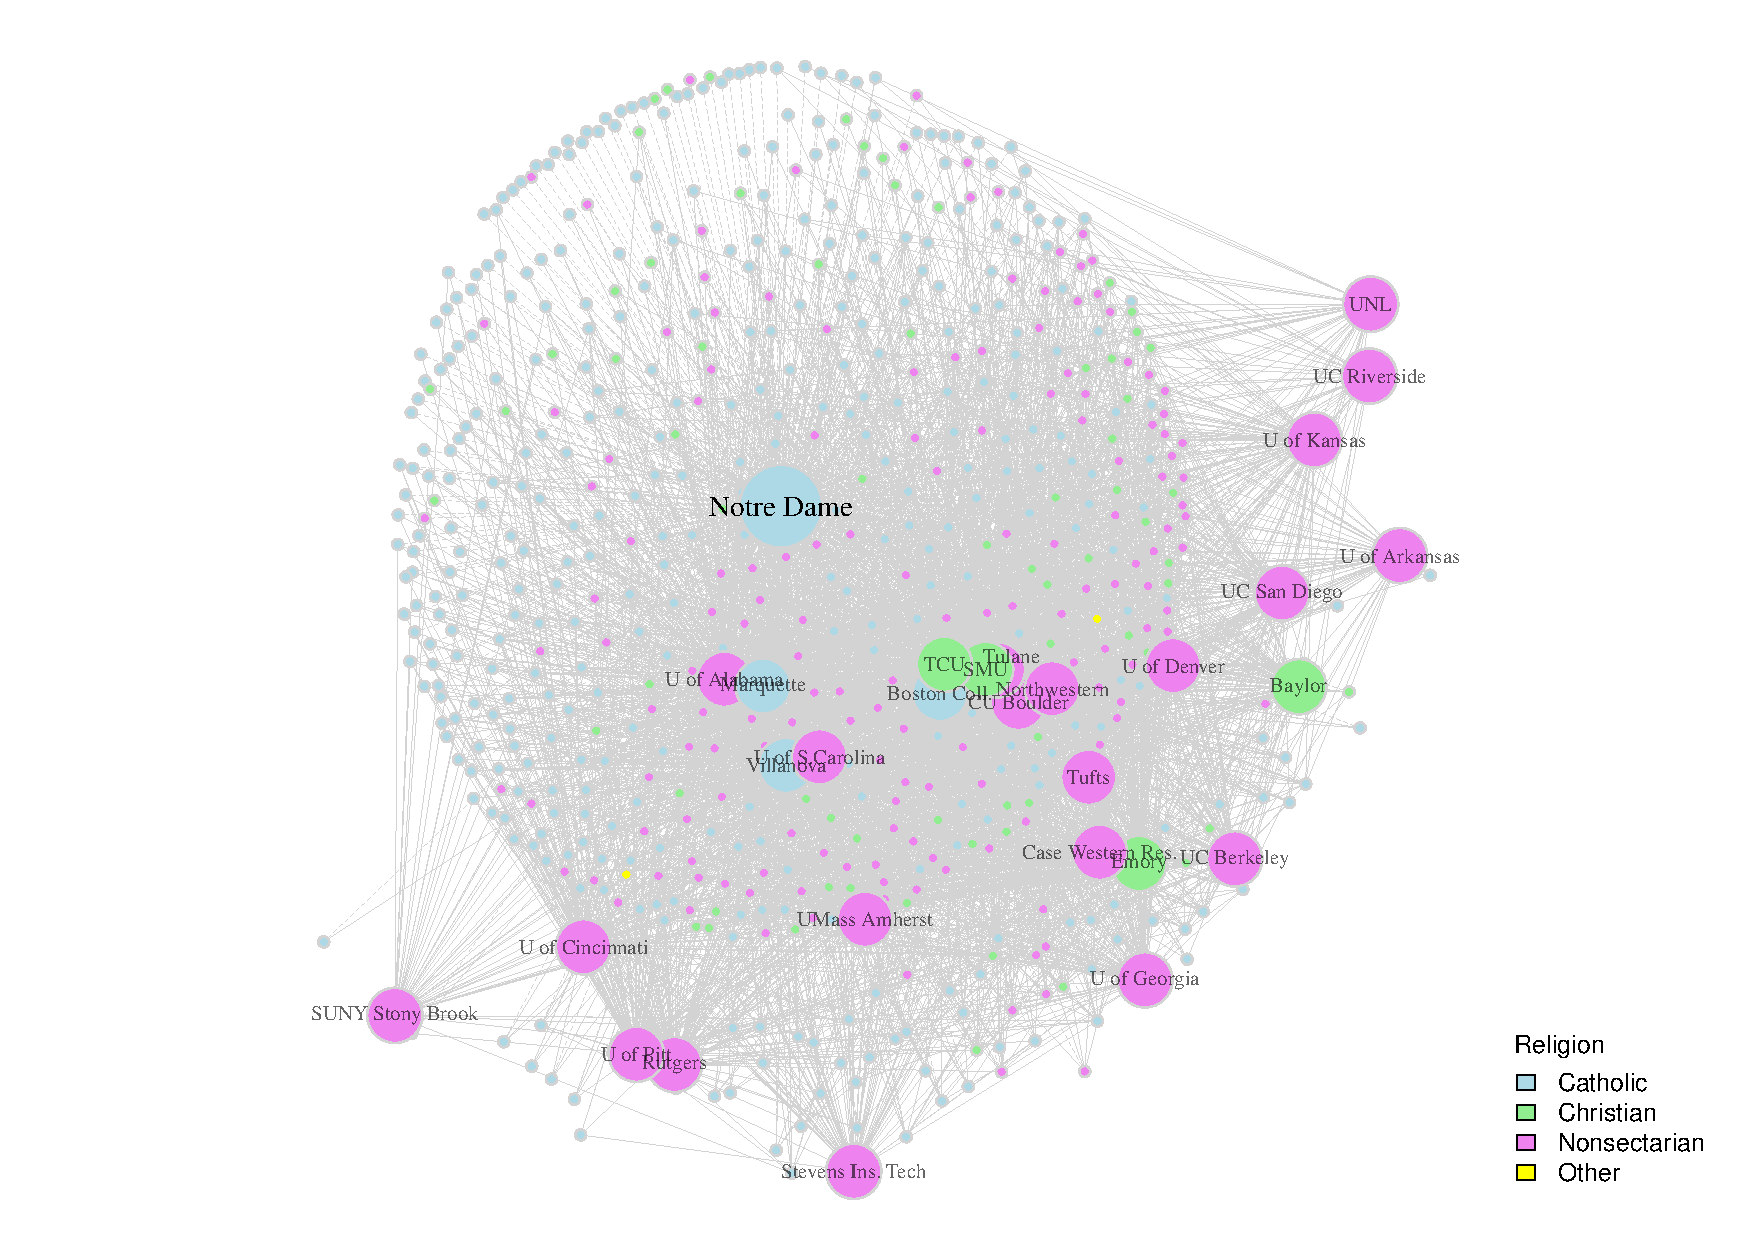
\includegraphics[width=2\linewidth]{../assets/figures/nd_religion} 

}

\caption{Order 2 ego network of University of Notre Dame, vertices colored by religion}\label{fig:nd-religion}
\end{figure}

\newpage

\begin{figure}

{\centering 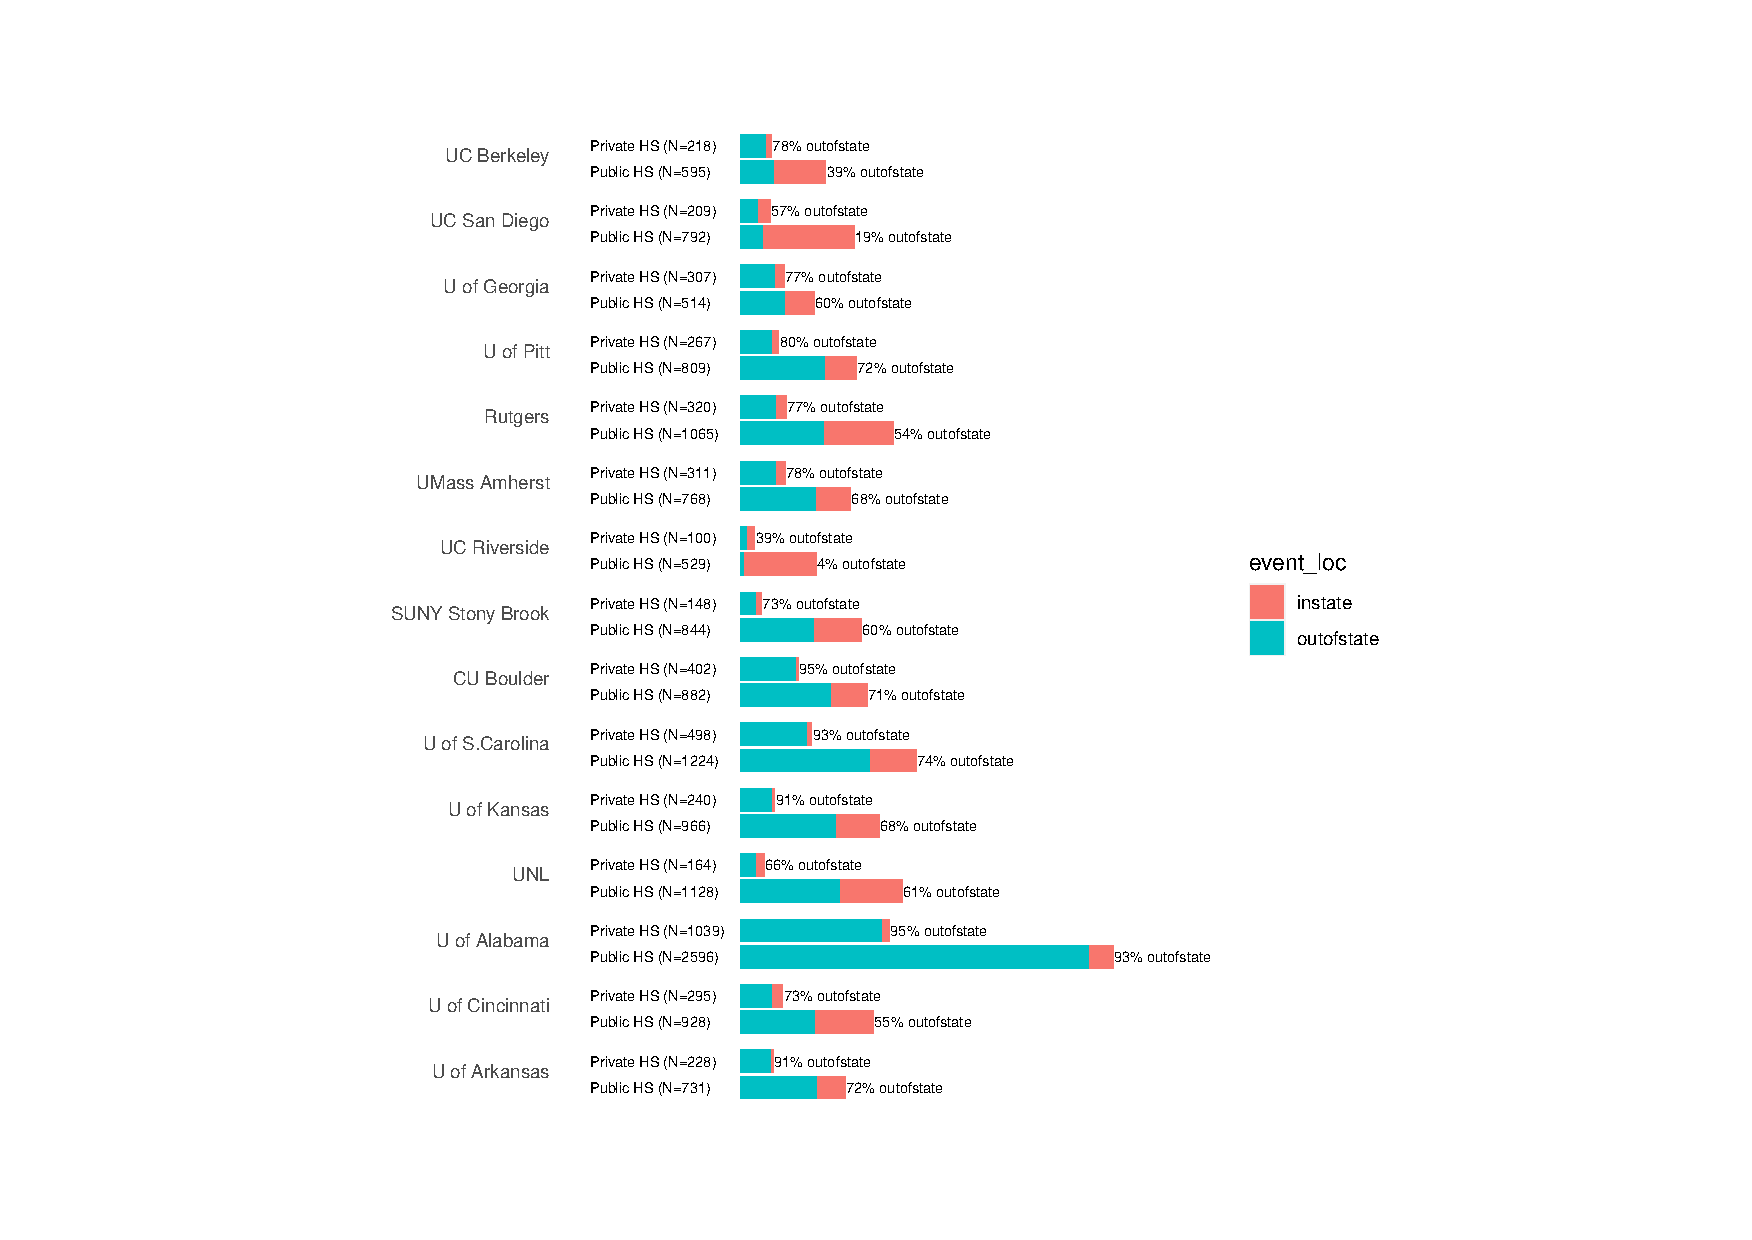
\includegraphics[width=2\linewidth]{../assets/figures/events_hs_count_pubu} 

}

\caption{Number of visits to public and private high schools by public research universities}\label{fig:events-hs-count-pubu}
\end{figure}

\newpage

\begin{figure}

{\centering 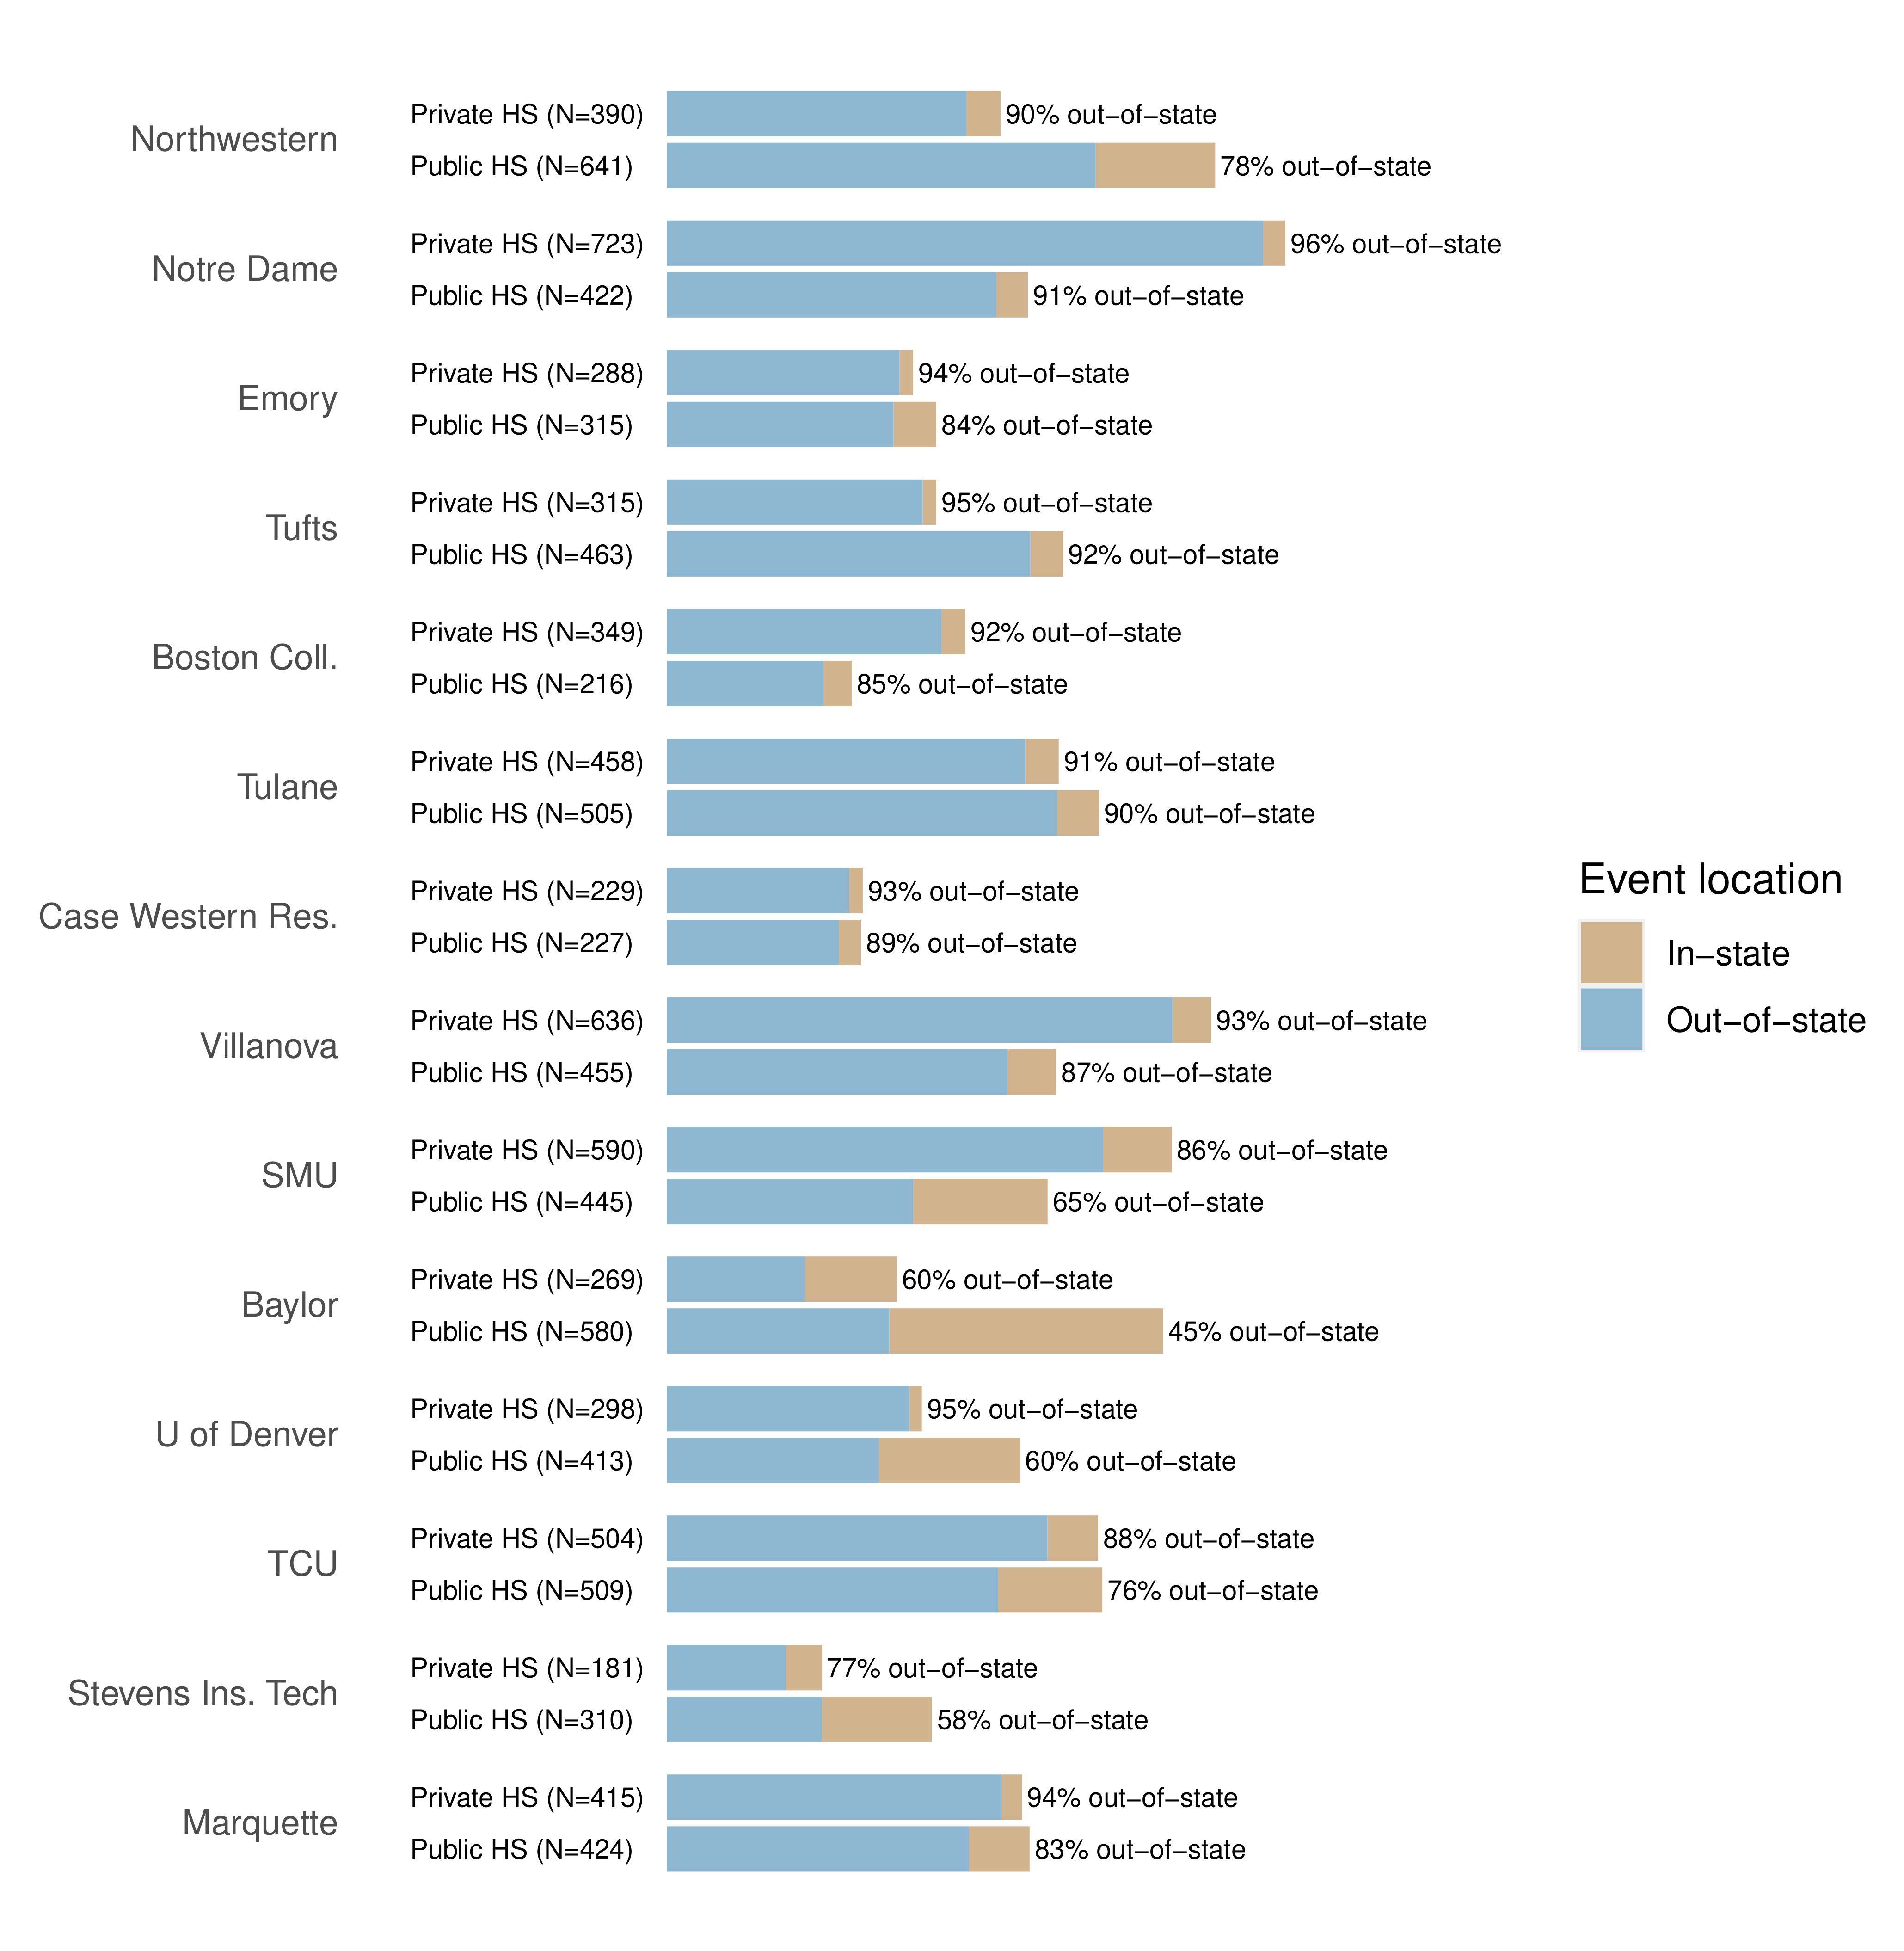
\includegraphics[width=2\linewidth]{../assets/figures/events_hs_count_privu} 

}

\caption{Number of visits to public and private high schools by selective private universities}\label{fig:events-hs-count-privu}
\end{figure}

\newpage

\begin{figure}

{\centering 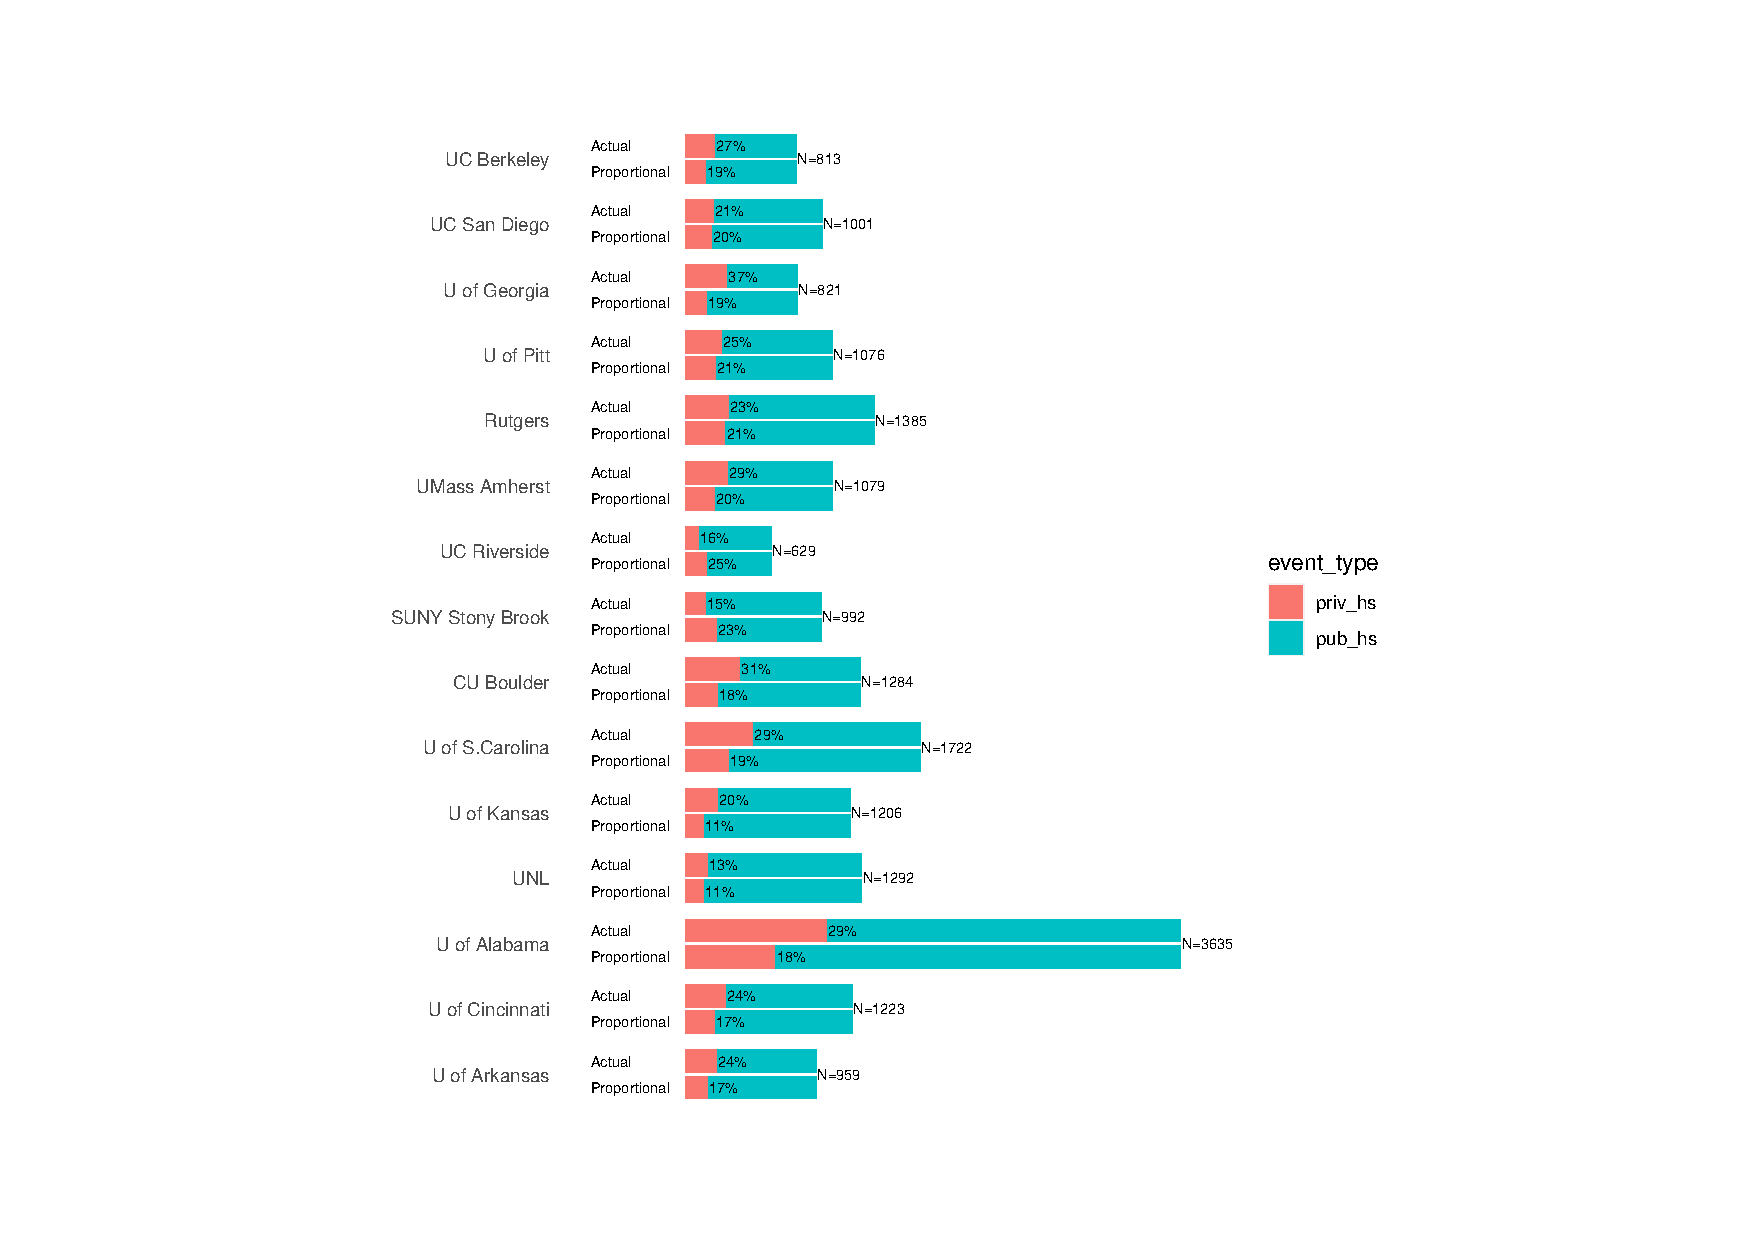
\includegraphics[width=2\linewidth]{../assets/figures/events_hs_actual_proportional_pubu} 

}

\caption{Actual versus proportional number of private school visits, public research universities}\label{fig:actual-proportional-pubu}
\end{figure}

\clearpage

\begin{figure}

{\centering 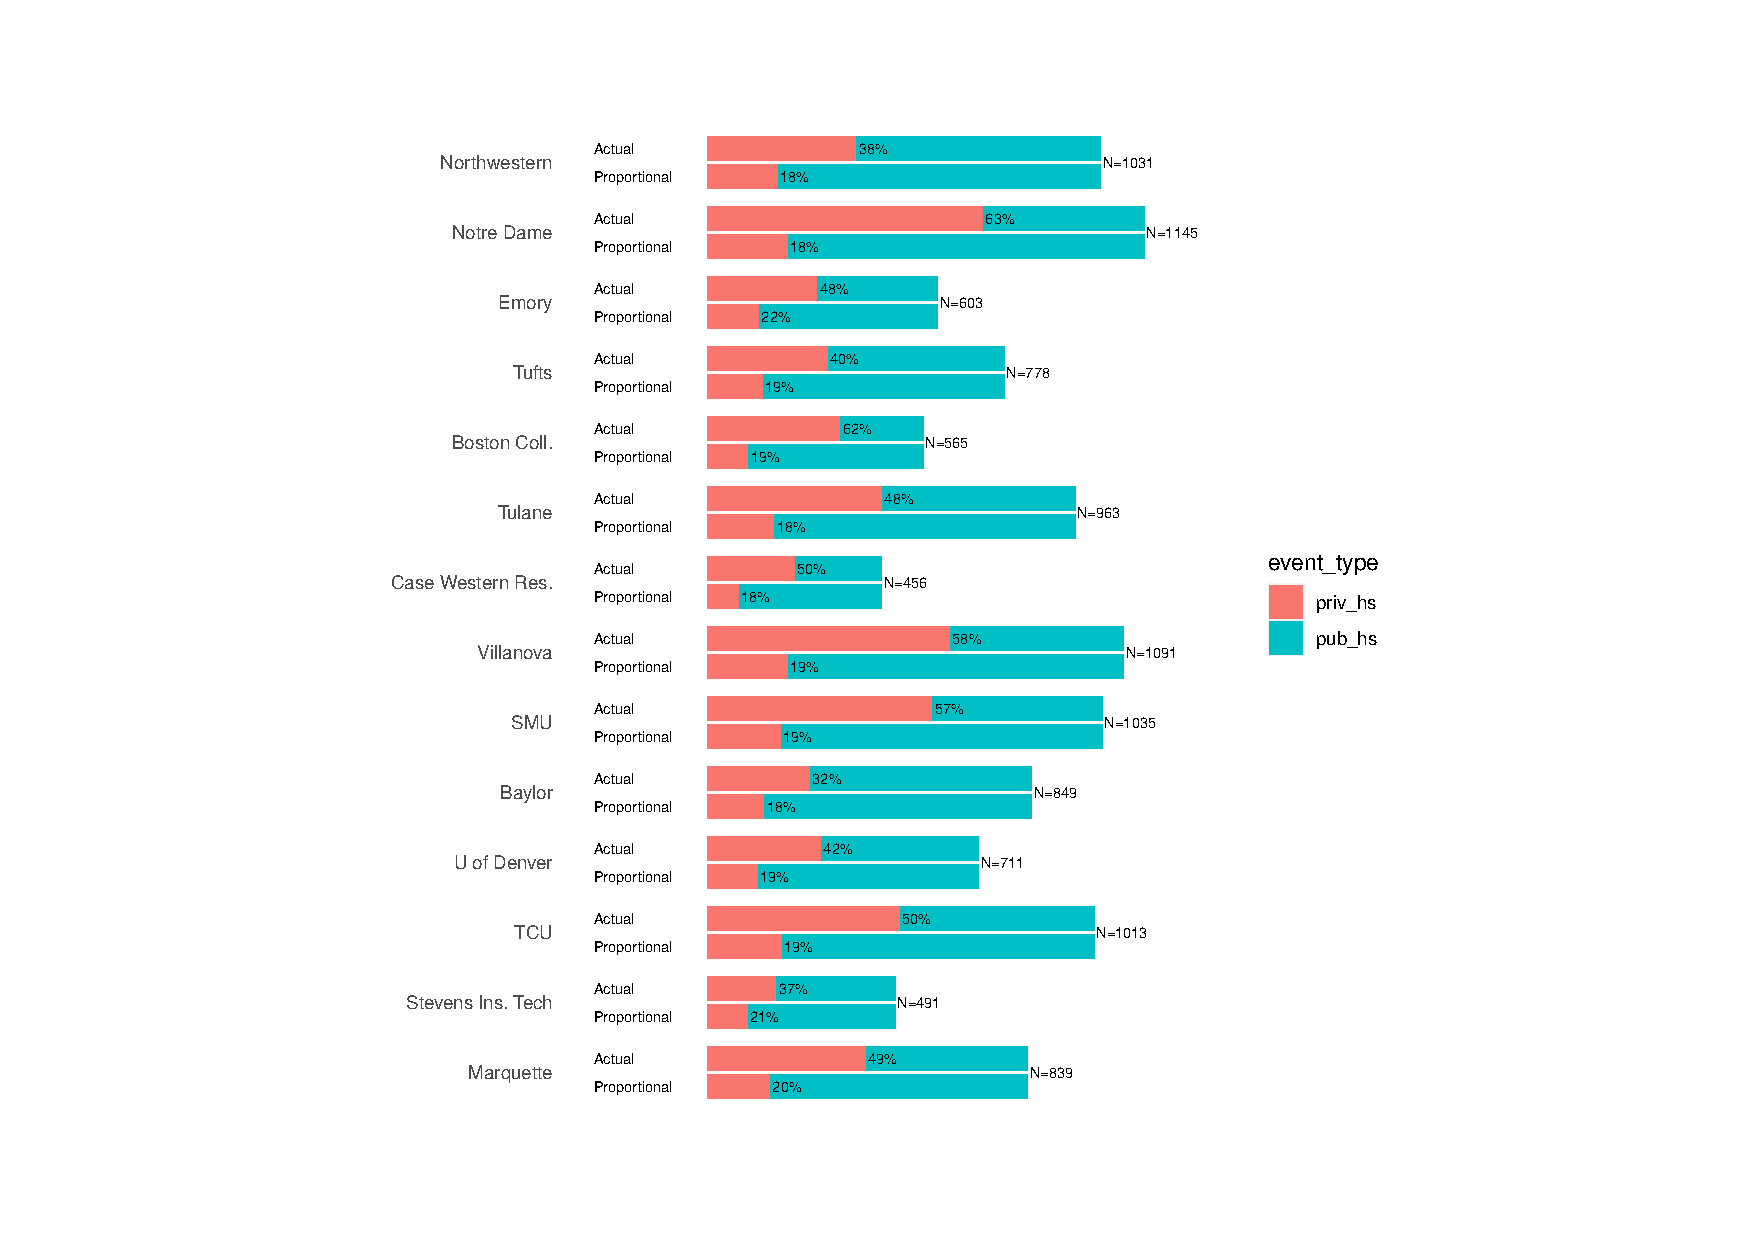
\includegraphics[width=2\linewidth]{../assets/figures/events_hs_actual_proportional_privu} 

}

\caption{Actual versus proportional number of private school visits, selective private universities}\label{fig:actual-proportional-privu}
\end{figure}

\newpage

\begin{figure}

{\centering 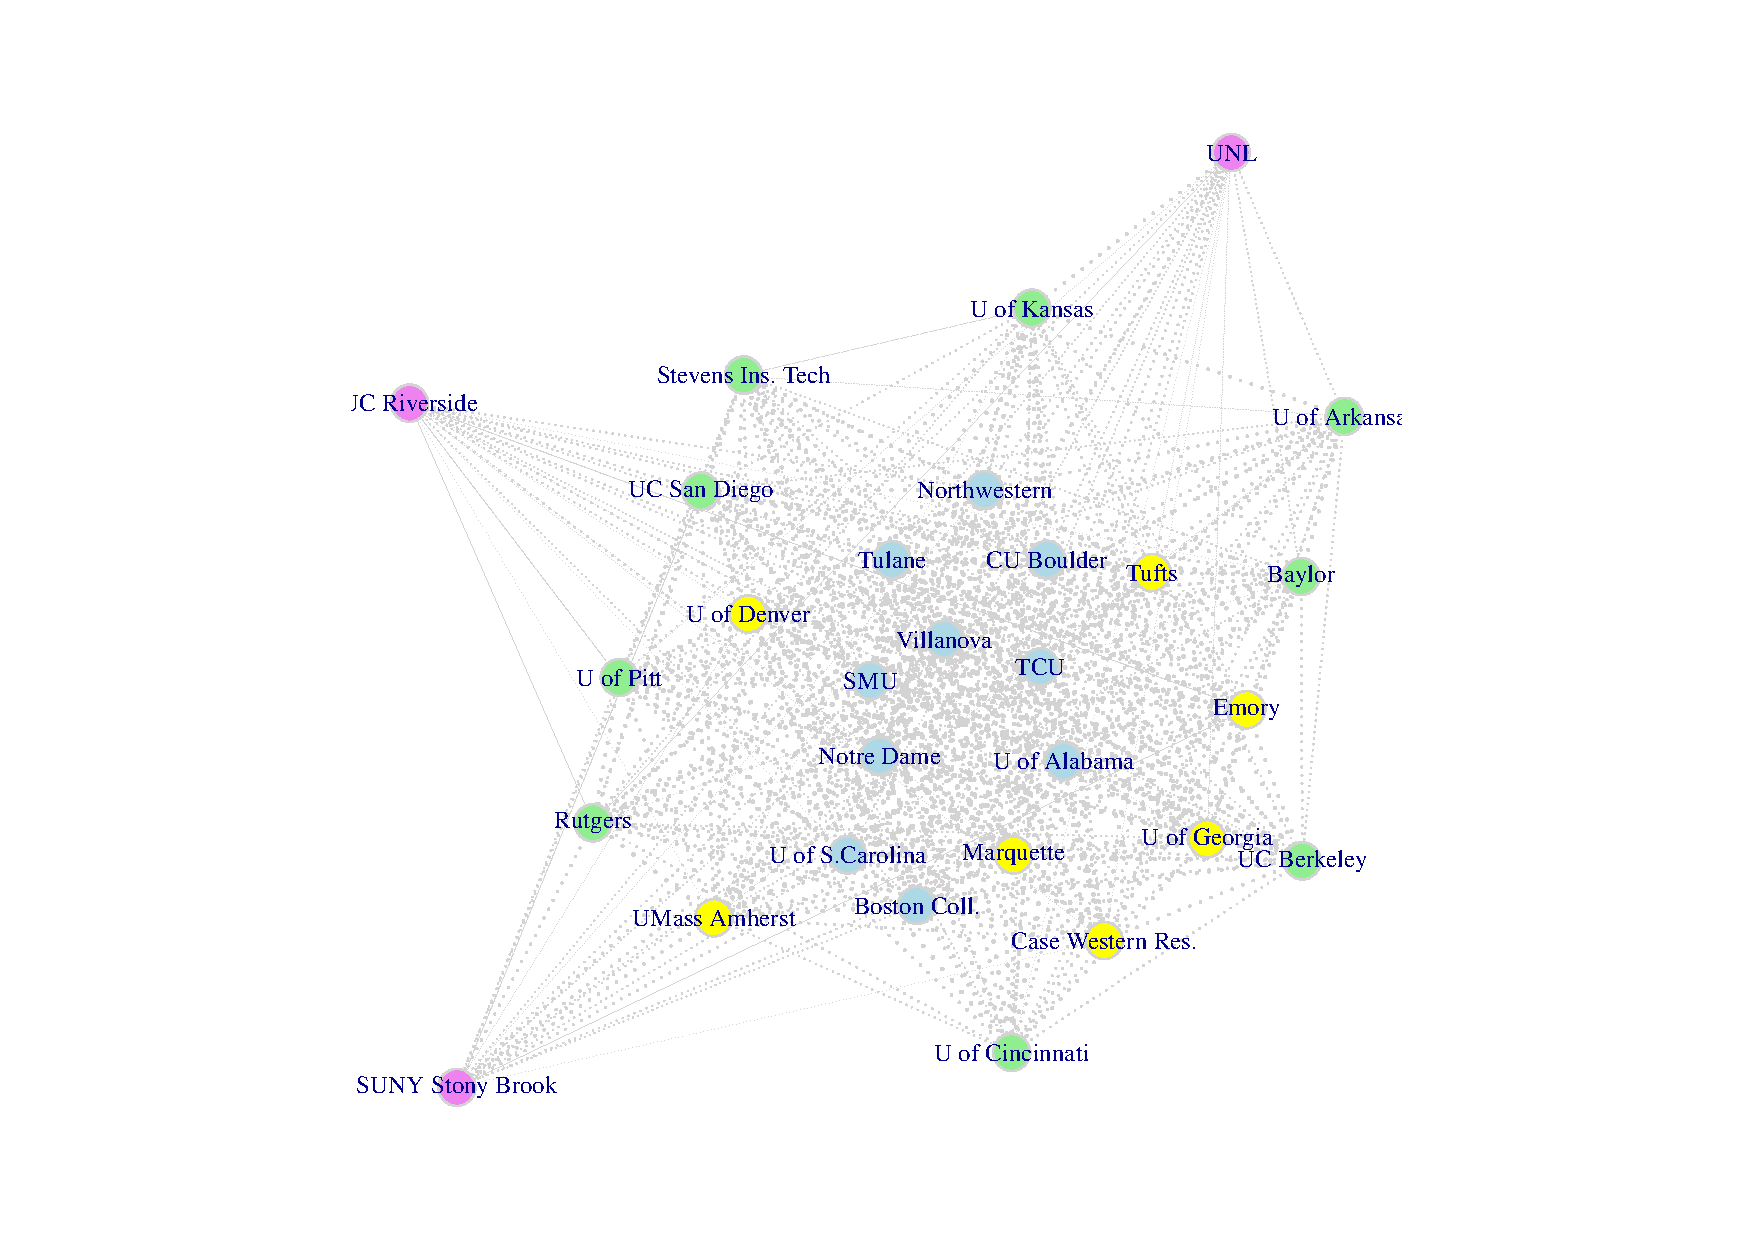
\includegraphics[width=2\linewidth]{../assets/figures/plot_1mode_u} 

}

\caption{One-mode network for public and private universities, colored by cluster}\label{fig:plot-1mode-u}
\end{figure}

\clearpage

\begin{figure}

{\centering 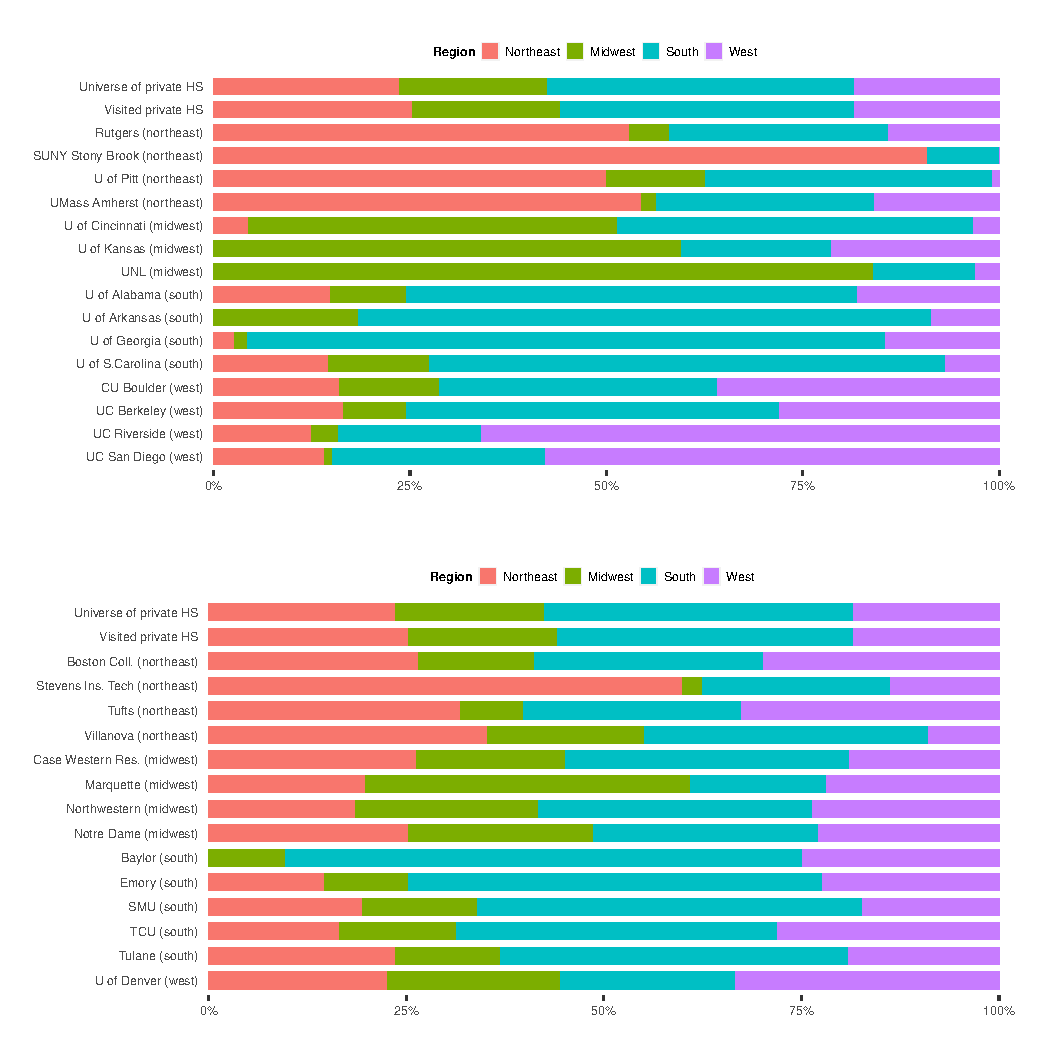
\includegraphics[width=2\linewidth]{../assets/figures/ego_network_region_pubu_privu} 

}

\caption{Geographic region of visited private high schools}\label{fig:region-pubu-privu}
\end{figure}

\newpage

\begin{figure}

{\centering 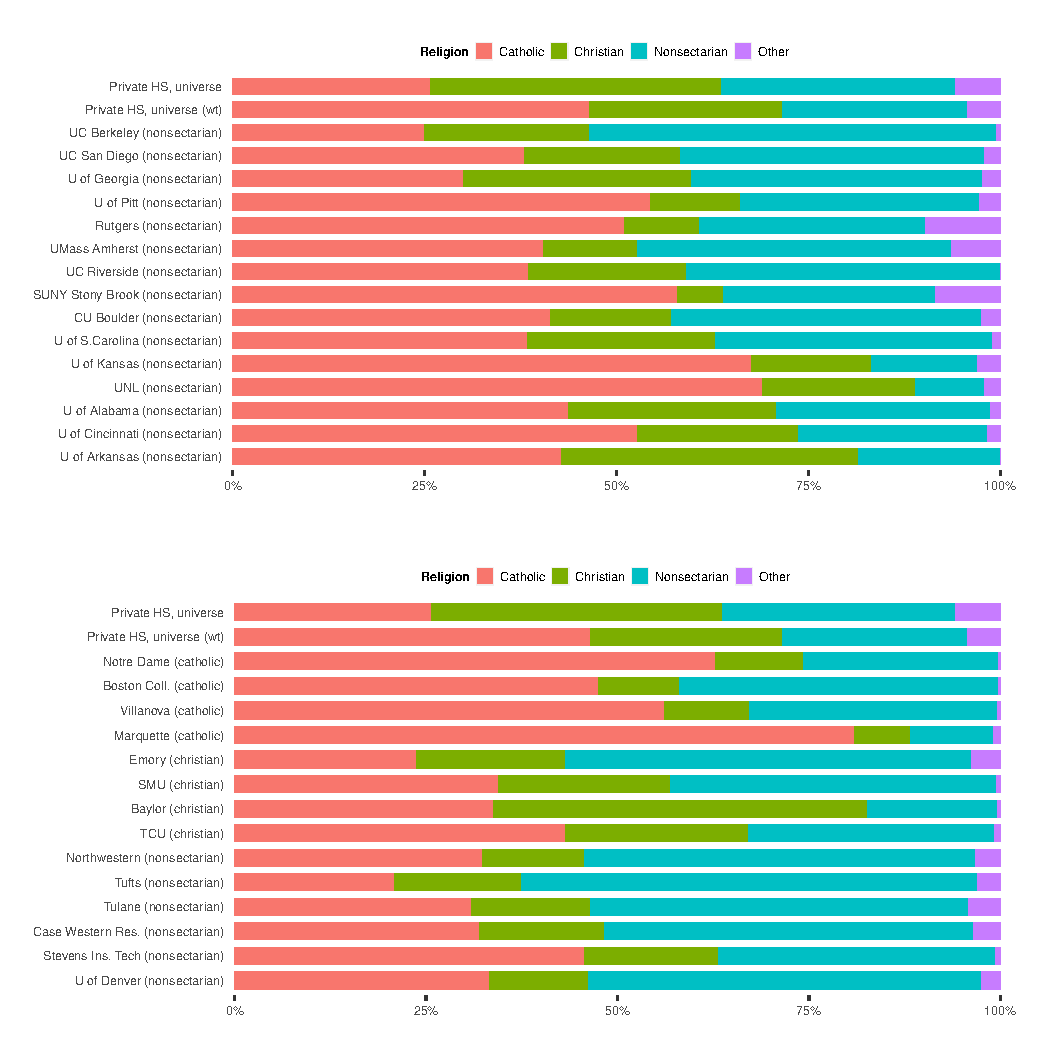
\includegraphics[width=2\linewidth]{../assets/figures/ego_network_religion_pubu_privu} 

}

\caption{Religious affiliation of visited private high schools}\label{fig:religion-pubu-privu}
\end{figure}

\newpage

\begin{figure}

{\centering 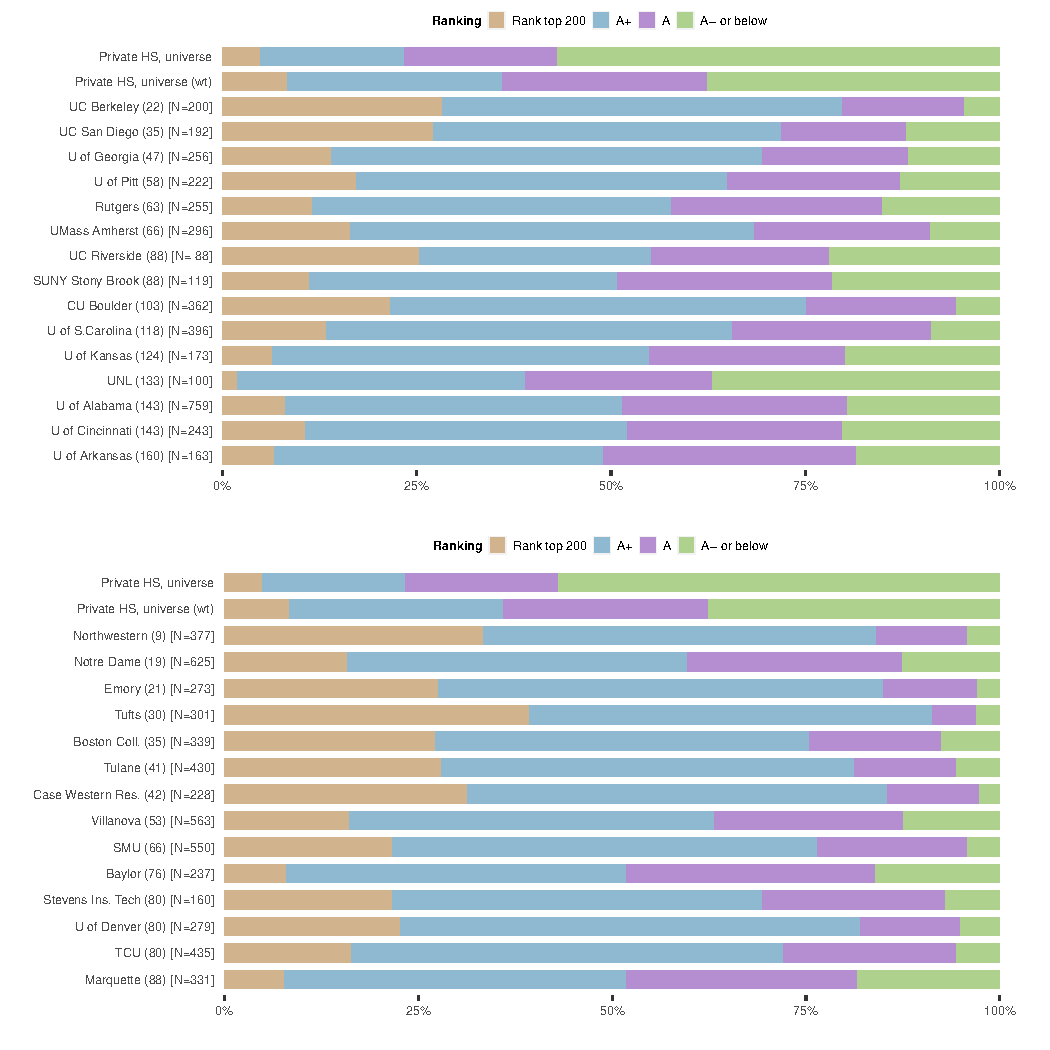
\includegraphics[width=2\linewidth]{../assets/figures/ego_network_rank_pubu_privu} 

}

\caption{High school ranking of visited private high schools}\label{fig:rank-pubu-privu}
\end{figure}

\newpage

\begin{figure}

{\centering 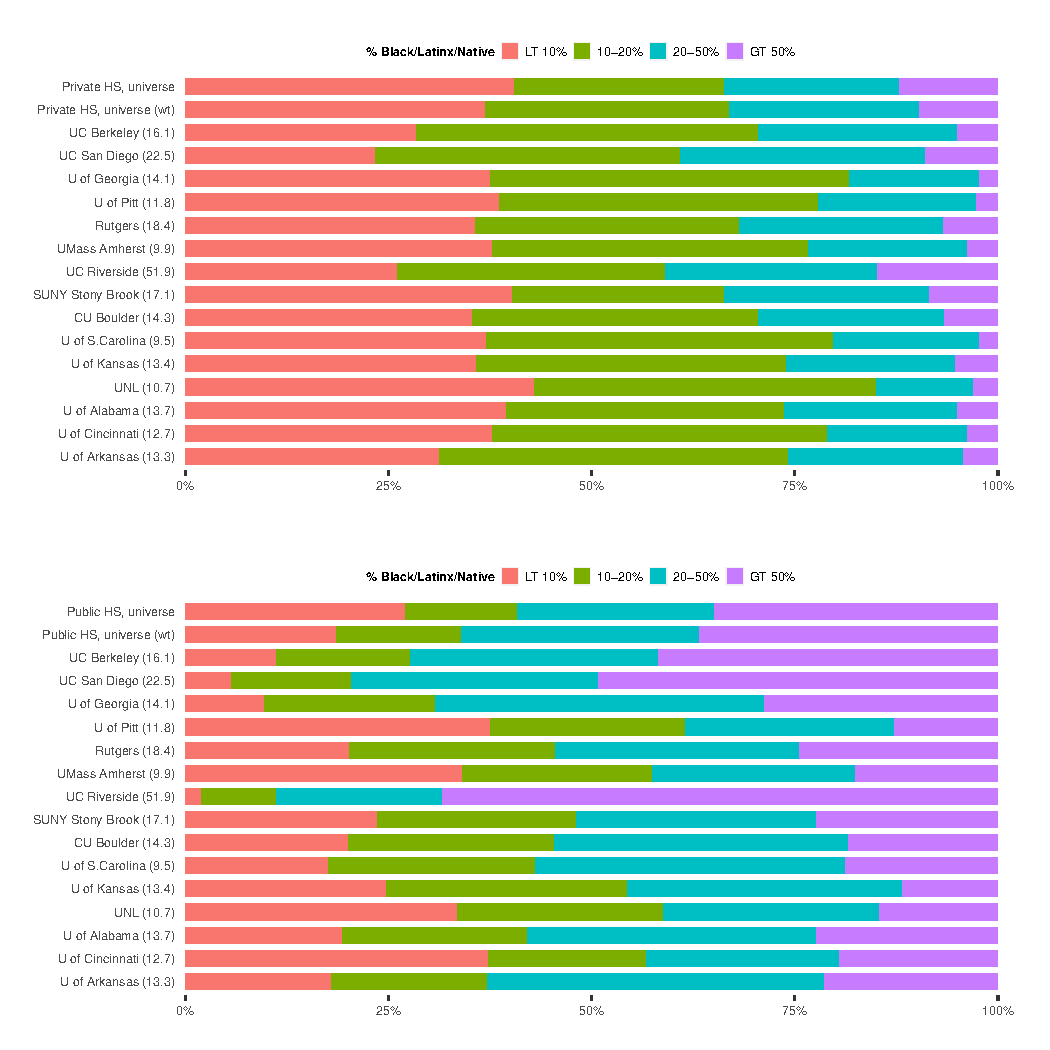
\includegraphics[width=2\linewidth]{../assets/figures/ego_network_race_pubu_privhs_pubhs} 

}

\caption{Percentage of students who identify as Black, Latinx, or Native at visited public high schools vs. visited private high schools, public research universities}\label{fig:race-pubu-privhs-pubhs}
\end{figure}

\newpage

\begin{figure}

{\centering 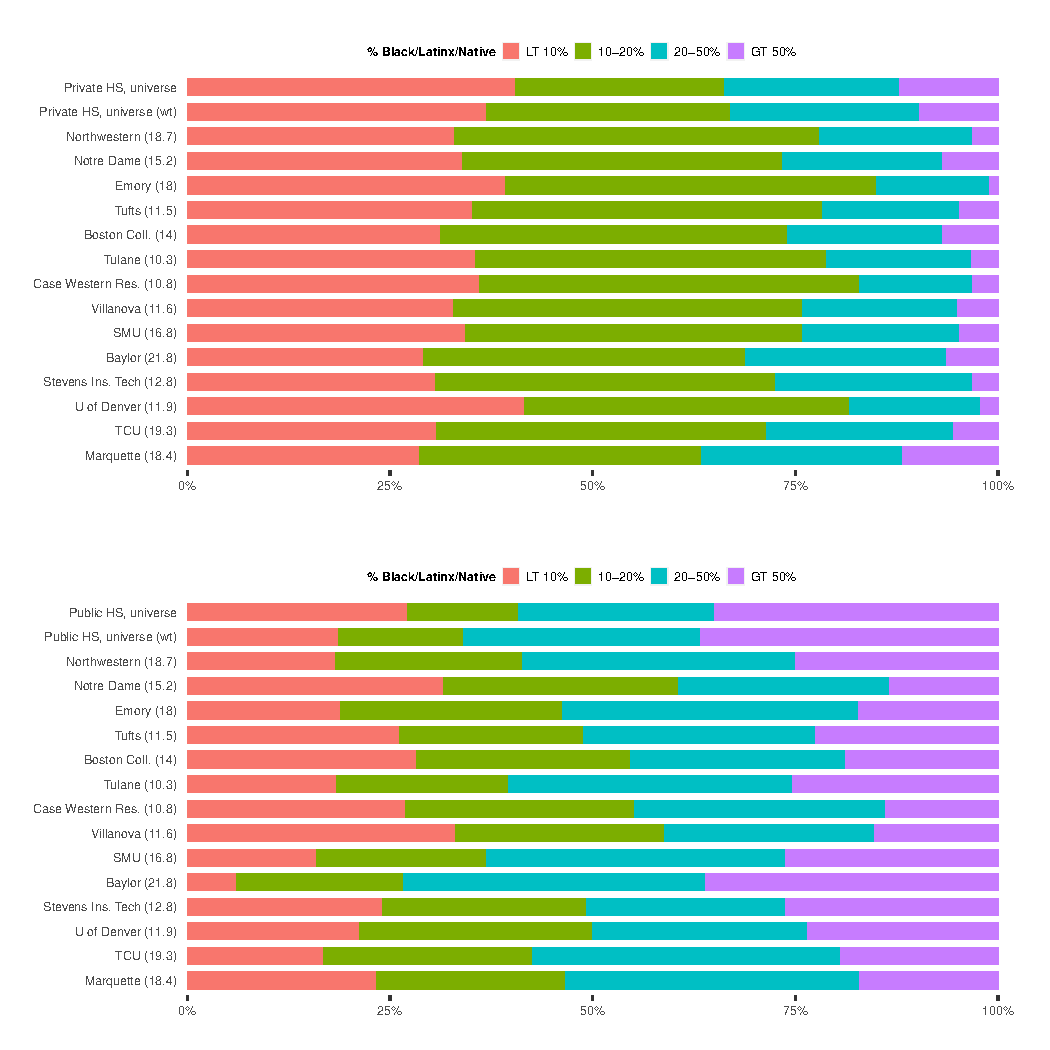
\includegraphics[width=2\linewidth]{../assets/figures/ego_network_race_privu_privhs_pubhs} 

}

\caption{Percentage of students who identify as Black, Latinx, or Native at visited public high schools vs. visited private high schools, selective private universities}\label{fig:race-privu-privhs-pubhs}
\end{figure}


\beginsupplement
\clearpage
\newpage

\begin{table}

\caption{\label{tab:pubu-count-matrix}One-mode public university count matrix}
\centering
\resizebox{\linewidth}{!}{
\fontsize{13}{15}\selectfont
\begin{tabular}[t]{l>{\centering\arraybackslash}p{6.5em}>{\centering\arraybackslash}p{7em}>{\centering\arraybackslash}p{5.5em}>{\centering\arraybackslash}p{7.5em}>{\centering\arraybackslash}p{6em}>{\centering\arraybackslash}p{5em}>{\centering\arraybackslash}p{7em}>{\centering\arraybackslash}p{5em}>{\centering\arraybackslash}p{6em}>{\centering\arraybackslash}p{6.5em}>{\centering\arraybackslash}p{5.5em}>{\centering\arraybackslash}p{6.5em}>{\centering\arraybackslash}p{8.8em}>{\centering\arraybackslash}p{5em}>{\centering\arraybackslash}p{6em}}
\toprule
  & U of Alabama (N=759) & U of S.Carolina (N=396) & CU Boulder (N=362) & UMass Amherst (N=296) & U of Georgia (N=256) & Rutgers (N=255) & U of Cincinnati (N=243) & U of Pitt (N=222) & UC Berkeley (N=200) & UC San Diego (N=192) & U of Kansas (N=173) & U of Arkansas (N=163) & SUNY Stony Brook (N=119) & UNL (N=100) & UC Riverside (N=88)\\
\midrule
U of Alabama (N=759) & 759 & 284 & 210 & 149 & 169 & 120 & 124 & 125 & 112 & 100 & 93 & 100 & 43 & 31 & 34\\
U of S.Carolina (N=396) & 284 & 396 & 155 & 108 & 140 & 74 & 110 & 99 & 84 & 59 & 58 & 57 & 27 & 20 & 19\\
CU Boulder (N=362) & 210 & 155 & 362 & 115 & 88 & 76 & 69 & 92 & 77 & 98 & 74 & 51 & 21 & 25 & 28\\
UMass Amherst (N=296) & 149 & 108 & 115 & 296 & 57 & 93 & 27 & 56 & 45 & 57 & 18 & 14 & 57 & 4 & 18\\
U of Georgia (N=256) & 169 & 140 & 88 & 57 & 256 & 24 & 73 & 48 & 64 & 38 & 39 & 59 & 7 & 13 & 16\\
Rutgers (N=255) & 120 & 74 & 76 & 93 & 24 & 255 & 35 & 74 & 41 & 43 & 20 & 5 & 48 & 10 & 10\\
U of Cincinnati (N=243) & 124 & 110 & 69 & 27 & 73 & 35 & 243 & 56 & 33 & 24 & 29 & 37 & 5 & 18 & 8\\
U of Pitt (N=222) & 125 & 99 & 92 & 56 & 48 & 74 & 56 & 222 & 41 & 28 & 32 & 26 & 27 & 15 & 11\\
UC Berkeley (N=200) & 112 & 84 & 77 & 45 & 64 & 41 & 33 & 41 & 200 & 61 & 30 & 26 & 9 & 8 & 20\\
UC San Diego (N=192) & 100 & 59 & 98 & 57 & 38 & 43 & 24 & 28 & 61 & 192 & 29 & 22 & 11 & 3 & 35\\
U of Kansas (N=173) & 93 & 58 & 74 & 18 & 39 & 20 & 29 & 32 & 30 & 29 & 173 & 62 & 0 & 61 & 8\\
U of Arkansas (N=163) & 100 & 57 & 51 & 14 & 59 & 5 & 37 & 26 & 26 & 22 & 62 & 163 & 1 & 24 & 9\\
SUNY Stony Brook (N=119) & 43 & 27 & 21 & 57 & 7 & 48 & 5 & 27 & 9 & 11 & 0 & 1 & 119 & 0 & 4\\
UNL (N=100) & 31 & 20 & 25 & 4 & 13 & 10 & 18 & 15 & 8 & 3 & 61 & 24 & 0 & 100 & 0\\
UC Riverside (N=88) & 34 & 19 & 28 & 18 & 16 & 10 & 8 & 11 & 20 & 35 & 8 & 9 & 4 & 0 & 88\\
\bottomrule
\end{tabular}}
\end{table}

\begin{table}

\caption{\label{tab:privu-count-matrix}One-mode private universities count matrix}
\centering
\resizebox{\linewidth}{!}{
\fontsize{13}{15}\selectfont
\begin{tabular}[t]{l>{\centering\arraybackslash}p{7em}>{\centering\arraybackslash}p{7em}>{\centering\arraybackslash}p{6em}>{\centering\arraybackslash}p{6em}>{\centering\arraybackslash}p{6em}>{\centering\arraybackslash}p{7em}>{\centering\arraybackslash}p{7em}>{\centering\arraybackslash}p{7em}>{\centering\arraybackslash}p{6em}>{\centering\arraybackslash}p{7em}>{\centering\arraybackslash}p{6em}>{\centering\arraybackslash}p{6em}>{\centering\arraybackslash}p{8.5em}>{\centering\arraybackslash}p{8.5em}}
\toprule
  & Notre Dame (N=625) & Villanova (N=563) & SMU (N=550) & TCU (N=435) & Tulane (N=430) & Northwestern (N=377) & Boston Coll. (N=339) & Marquette (N=331) & Tufts (N=301) & U of Denver (N=279) & Emory (N=273) & Baylor (N=237) & Case Western Res. (N=228) & Stevens Ins. Tech (N=160)\\
\midrule
Notre Dame (N=625) & 625 & 338 & 293 & 253 & 223 & 224 & 235 & 231 & 177 & 164 & 145 & 99 & 133 & 79\\
Villanova (N=563) & 338 & 563 & 291 & 224 & 218 & 214 & 208 & 205 & 161 & 143 & 147 & 101 & 142 & 103\\
SMU (N=550) & 293 & 291 & 550 & 290 & 275 & 243 & 218 & 151 & 189 & 177 & 176 & 154 & 134 & 88\\
TCU (N=435) & 253 & 224 & 290 & 435 & 199 & 177 & 168 & 150 & 141 & 151 & 122 & 133 & 98 & 66\\
Tulane (N=430) & 223 & 218 & 275 & 199 & 430 & 219 & 173 & 103 & 190 & 142 & 143 & 79 & 131 & 56\\
Northwestern (N=377) & 224 & 214 & 243 & 177 & 219 & 377 & 172 & 114 & 169 & 139 & 128 & 75 & 122 & 55\\
Boston Coll. (N=339) & 235 & 208 & 218 & 168 & 173 & 172 & 339 & 133 & 158 & 135 & 113 & 64 & 100 & 60\\
Marquette (N=331) & 231 & 205 & 151 & 150 & 103 & 114 & 133 & 331 & 77 & 97 & 52 & 62 & 66 & 43\\
Tufts (N=301) & 177 & 161 & 189 & 141 & 190 & 169 & 158 & 77 & 301 & 114 & 117 & 52 & 108 & 66\\
U of Denver (N=279) & 164 & 143 & 177 & 151 & 142 & 139 & 135 & 97 & 114 & 279 & 82 & 57 & 72 & 44\\
Emory (N=273) & 145 & 147 & 176 & 122 & 143 & 128 & 113 & 52 & 117 & 82 & 273 & 39 & 98 & 42\\
Baylor (N=237) & 99 & 101 & 154 & 133 & 79 & 75 & 64 & 62 & 52 & 57 & 39 & 237 & 50 & 23\\
Case Western Res. (N=228) & 133 & 142 & 134 & 98 & 131 & 122 & 100 & 66 & 108 & 72 & 98 & 50 & 228 & 41\\
Stevens Ins. Tech (N=160) & 79 & 103 & 88 & 66 & 56 & 55 & 60 & 43 & 66 & 44 & 42 & 23 & 41 & 160\\
\bottomrule
\end{tabular}}
\end{table}

\newpage

\begin{figure}

{\centering 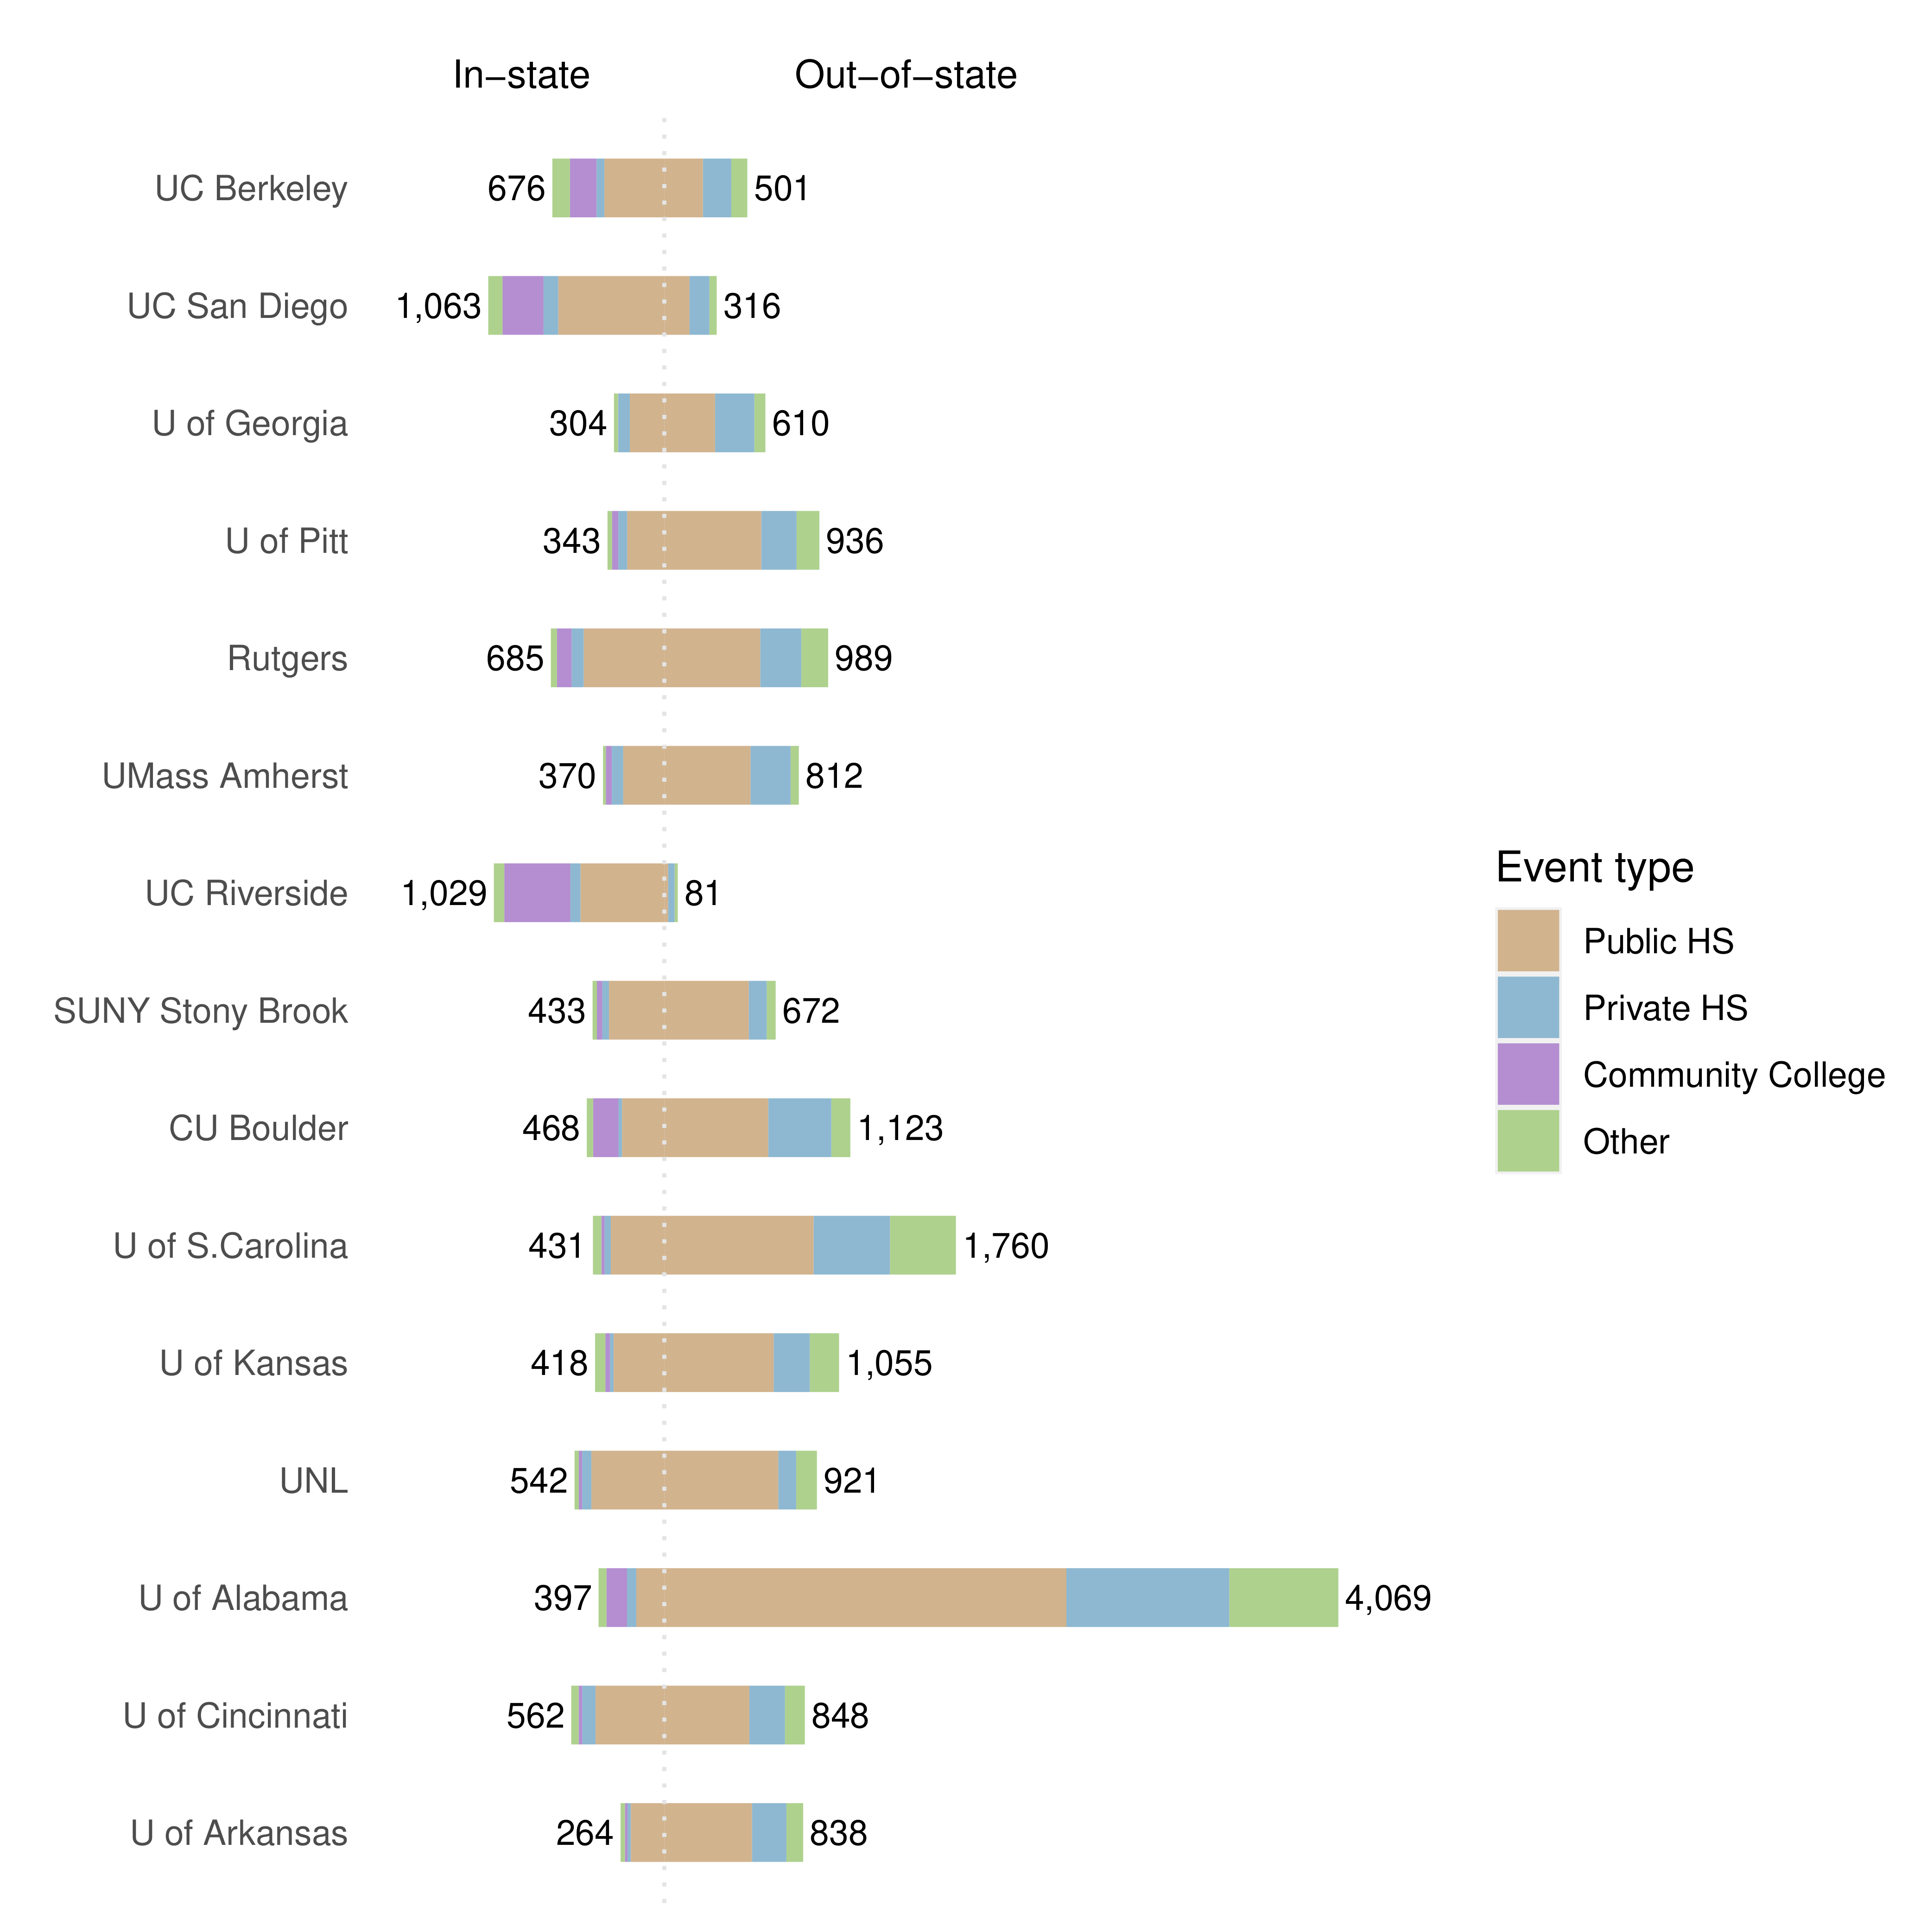
\includegraphics[width=2\linewidth]{../assets/figures/events_count_pubu} 

}

\caption{Number of visits by type and in-state vs. out-of-state, public research universities}\label{fig:events-count-pubu}
\end{figure}

\newpage

\begin{figure}

{\centering 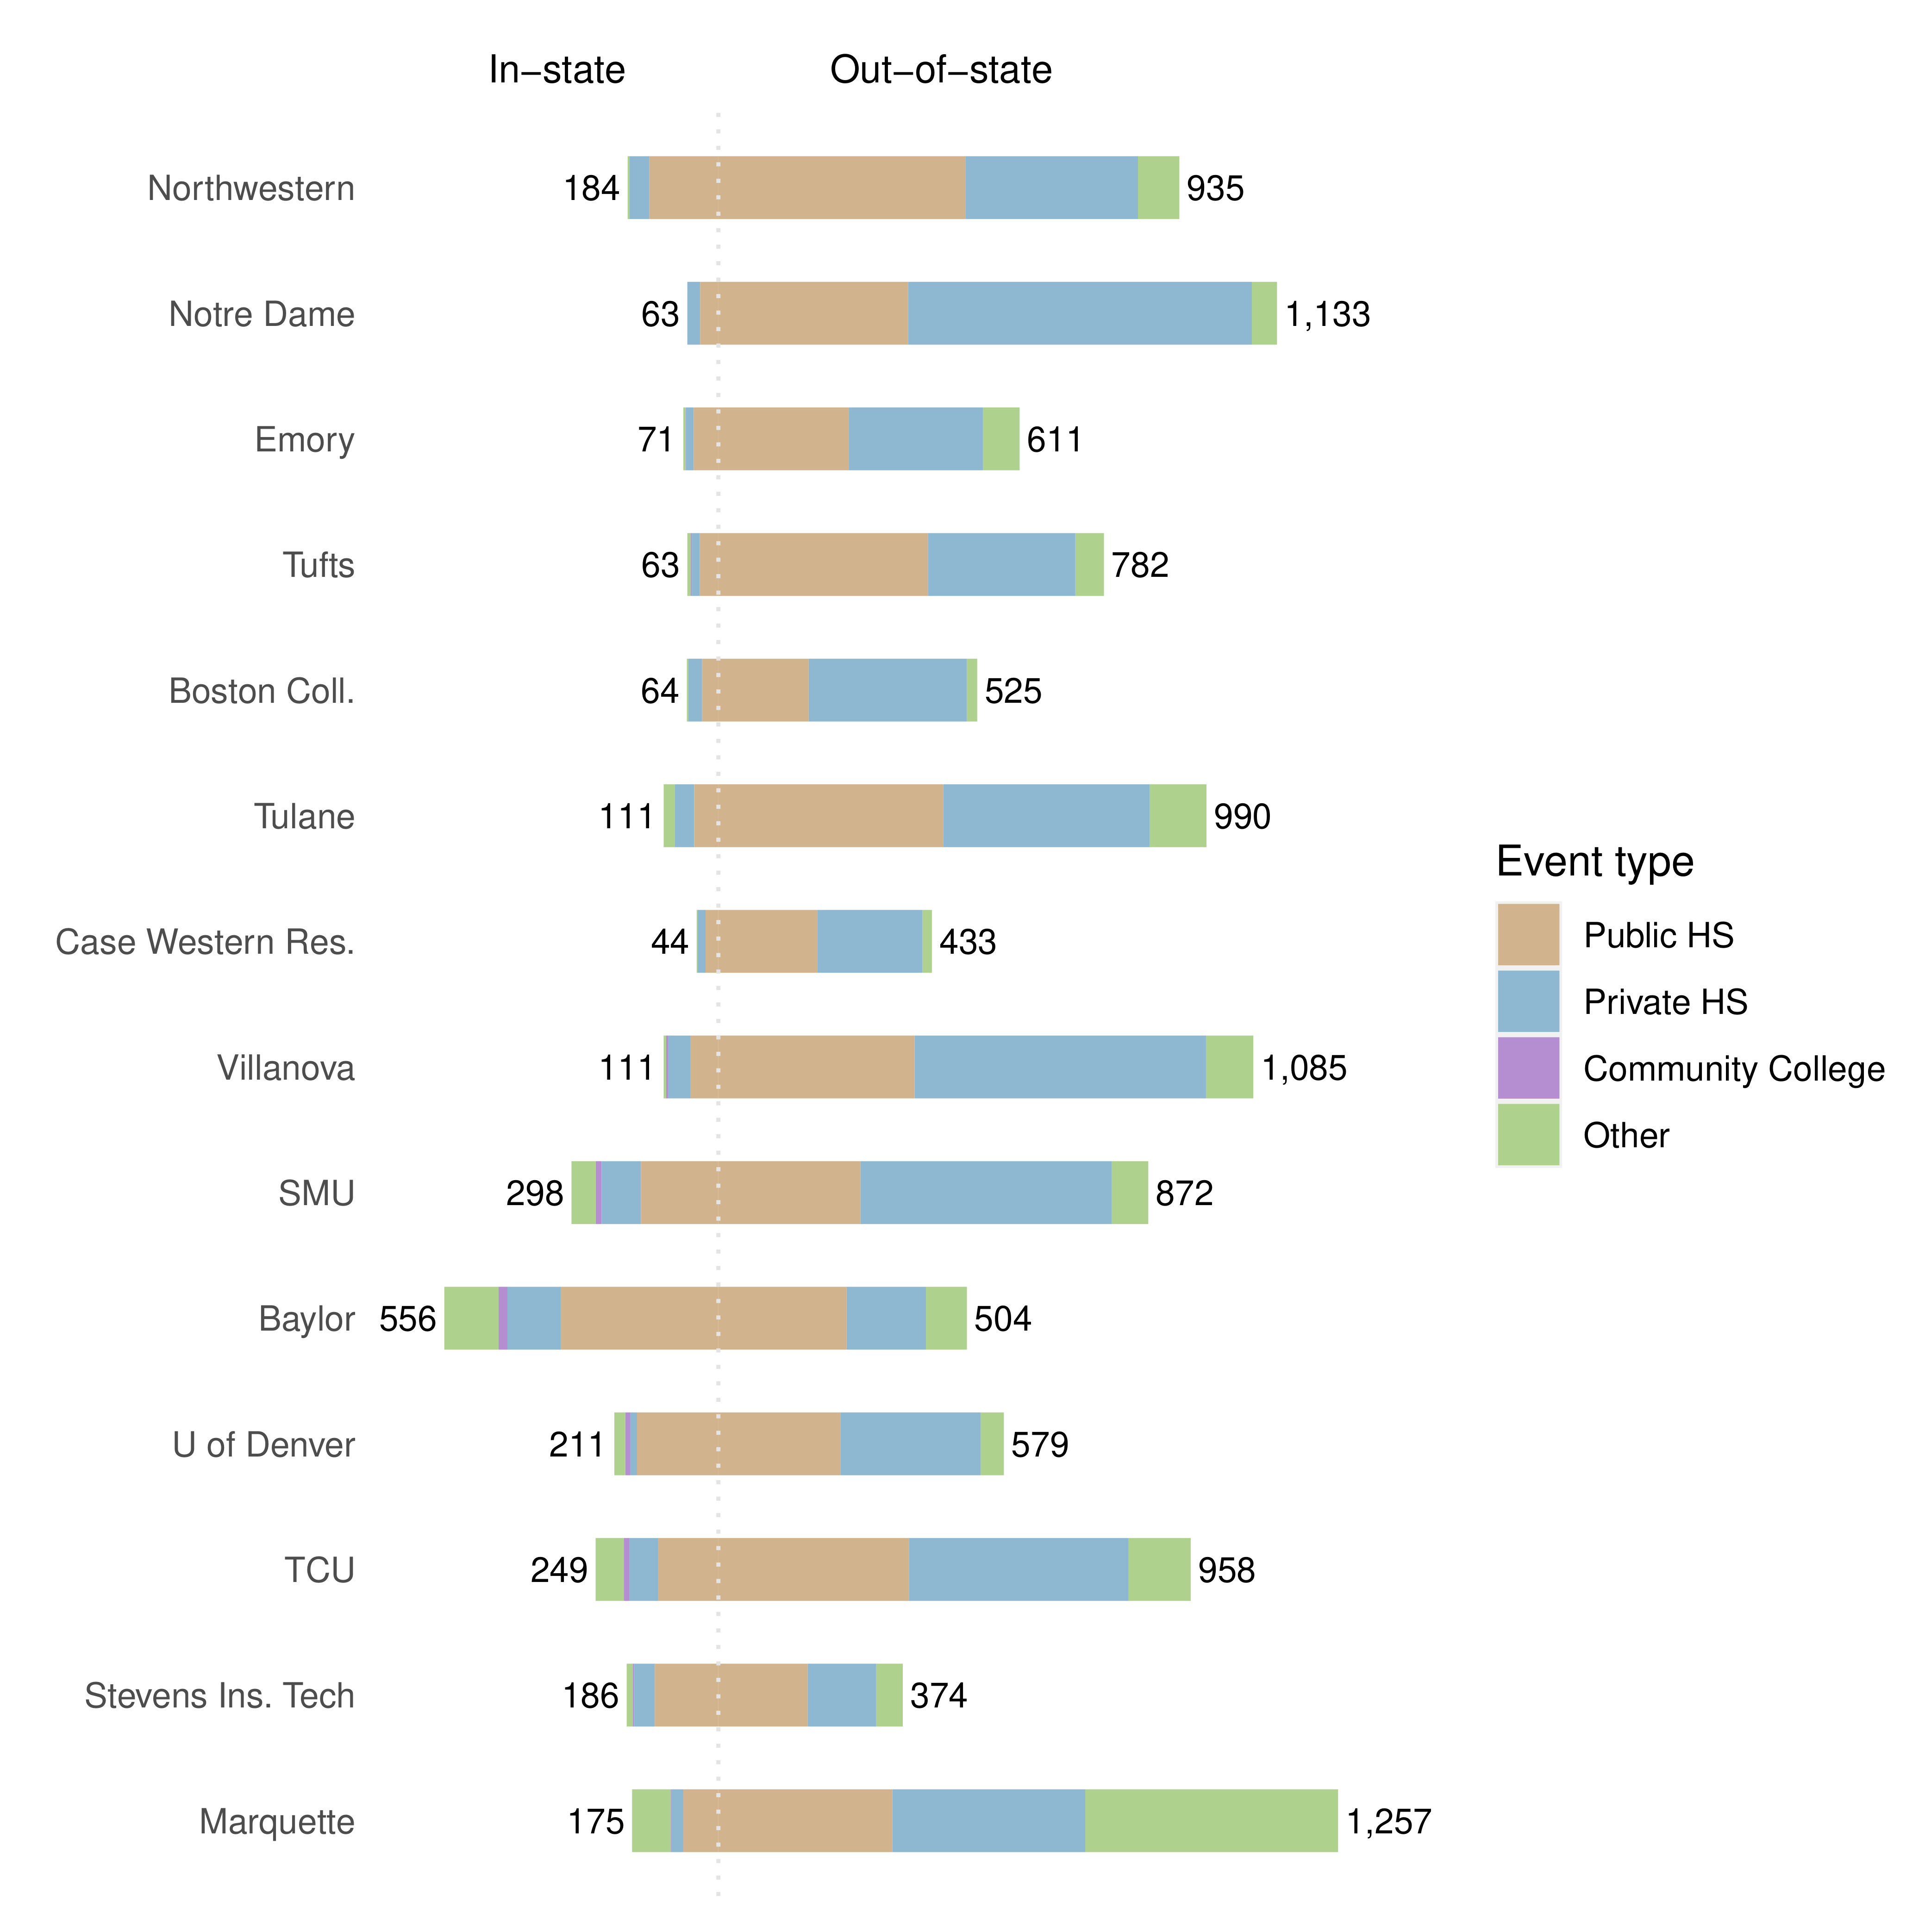
\includegraphics[width=2\linewidth]{../assets/figures/events_count_privu} 

}

\caption{Number of visits by type and in-state vs. out-of-state, selective private universities}\label{fig:events-count-privu}
\end{figure}

\newpage

\begin{figure}

{\centering 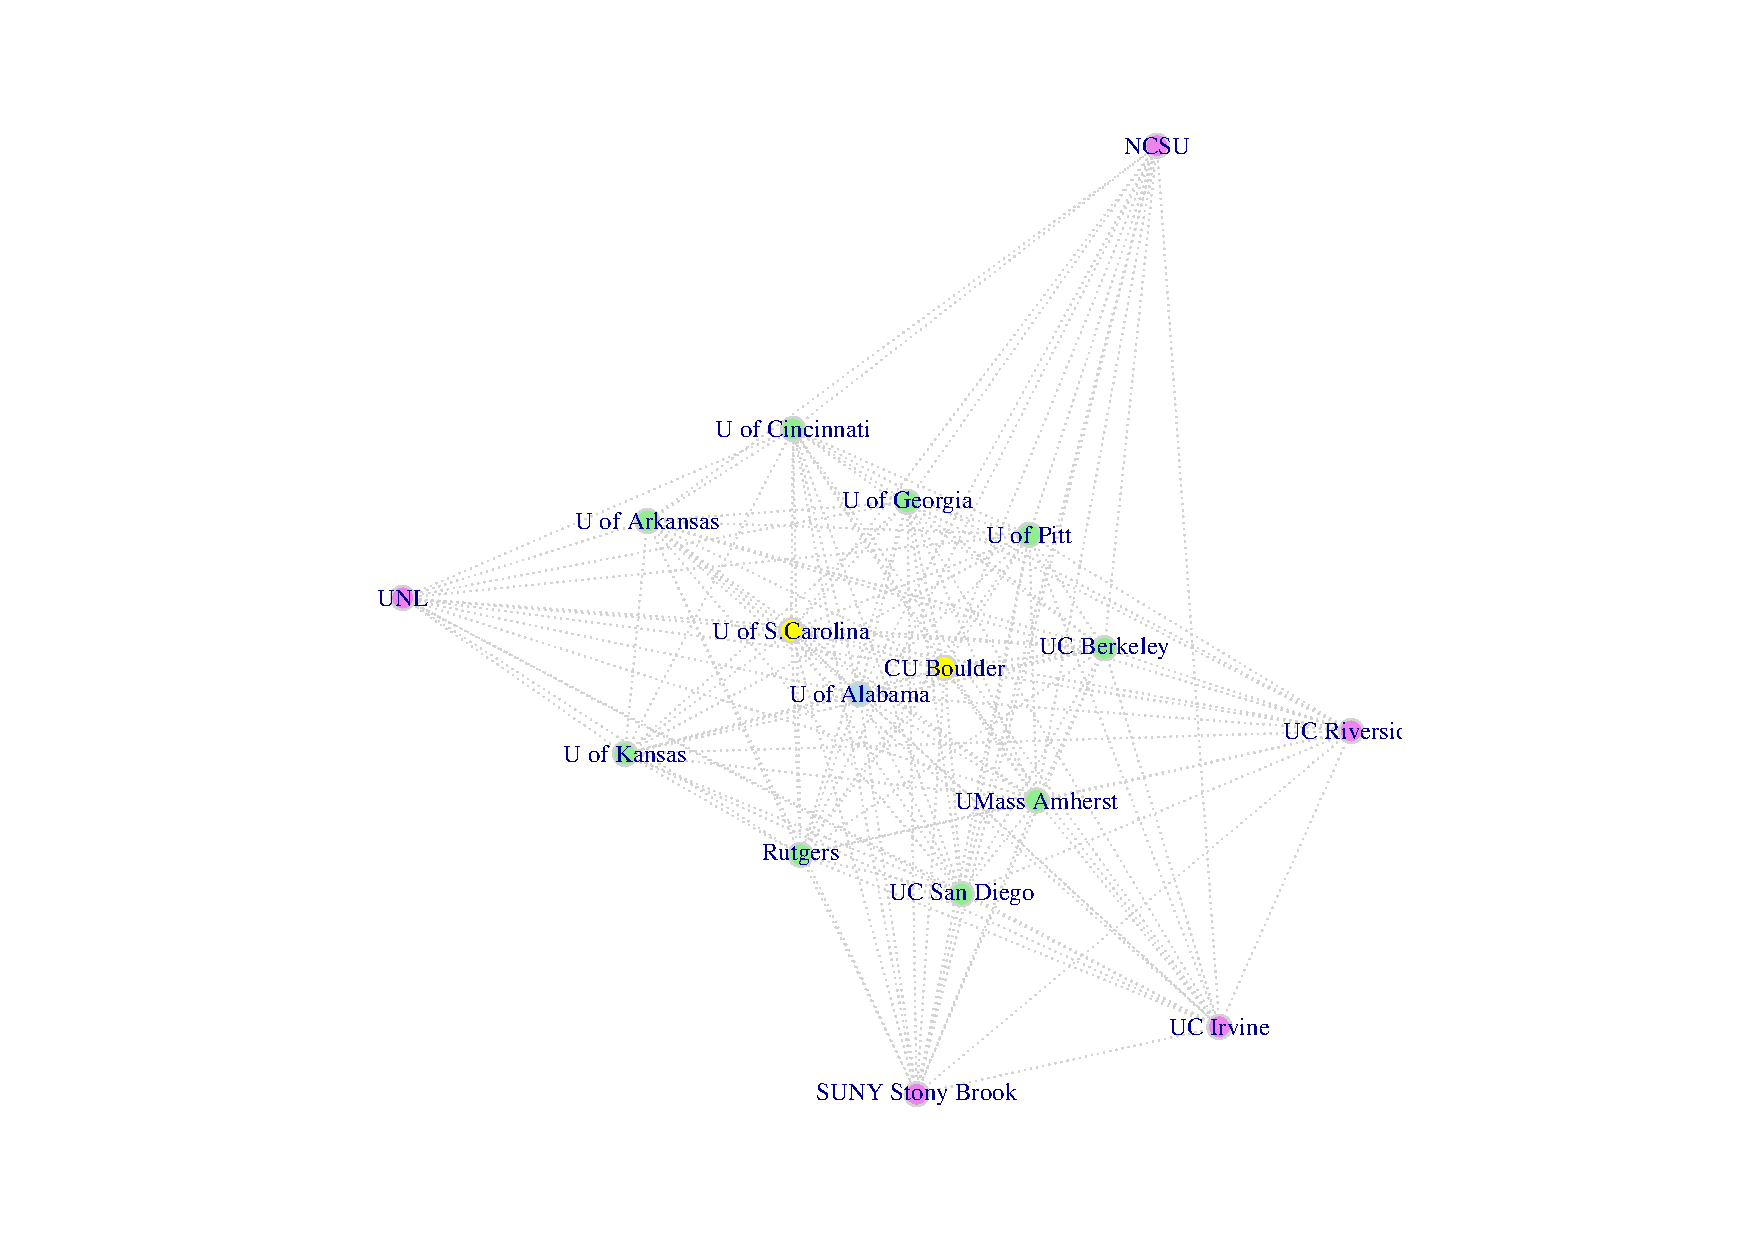
\includegraphics[width=2\linewidth]{../assets/figures/plot_1mode_pubu} 

}

\caption{One-mode network for public institutions, colored by cluster}\label{fig:plot-1mode-pubu}
\end{figure}

\begin{figure}

{\centering 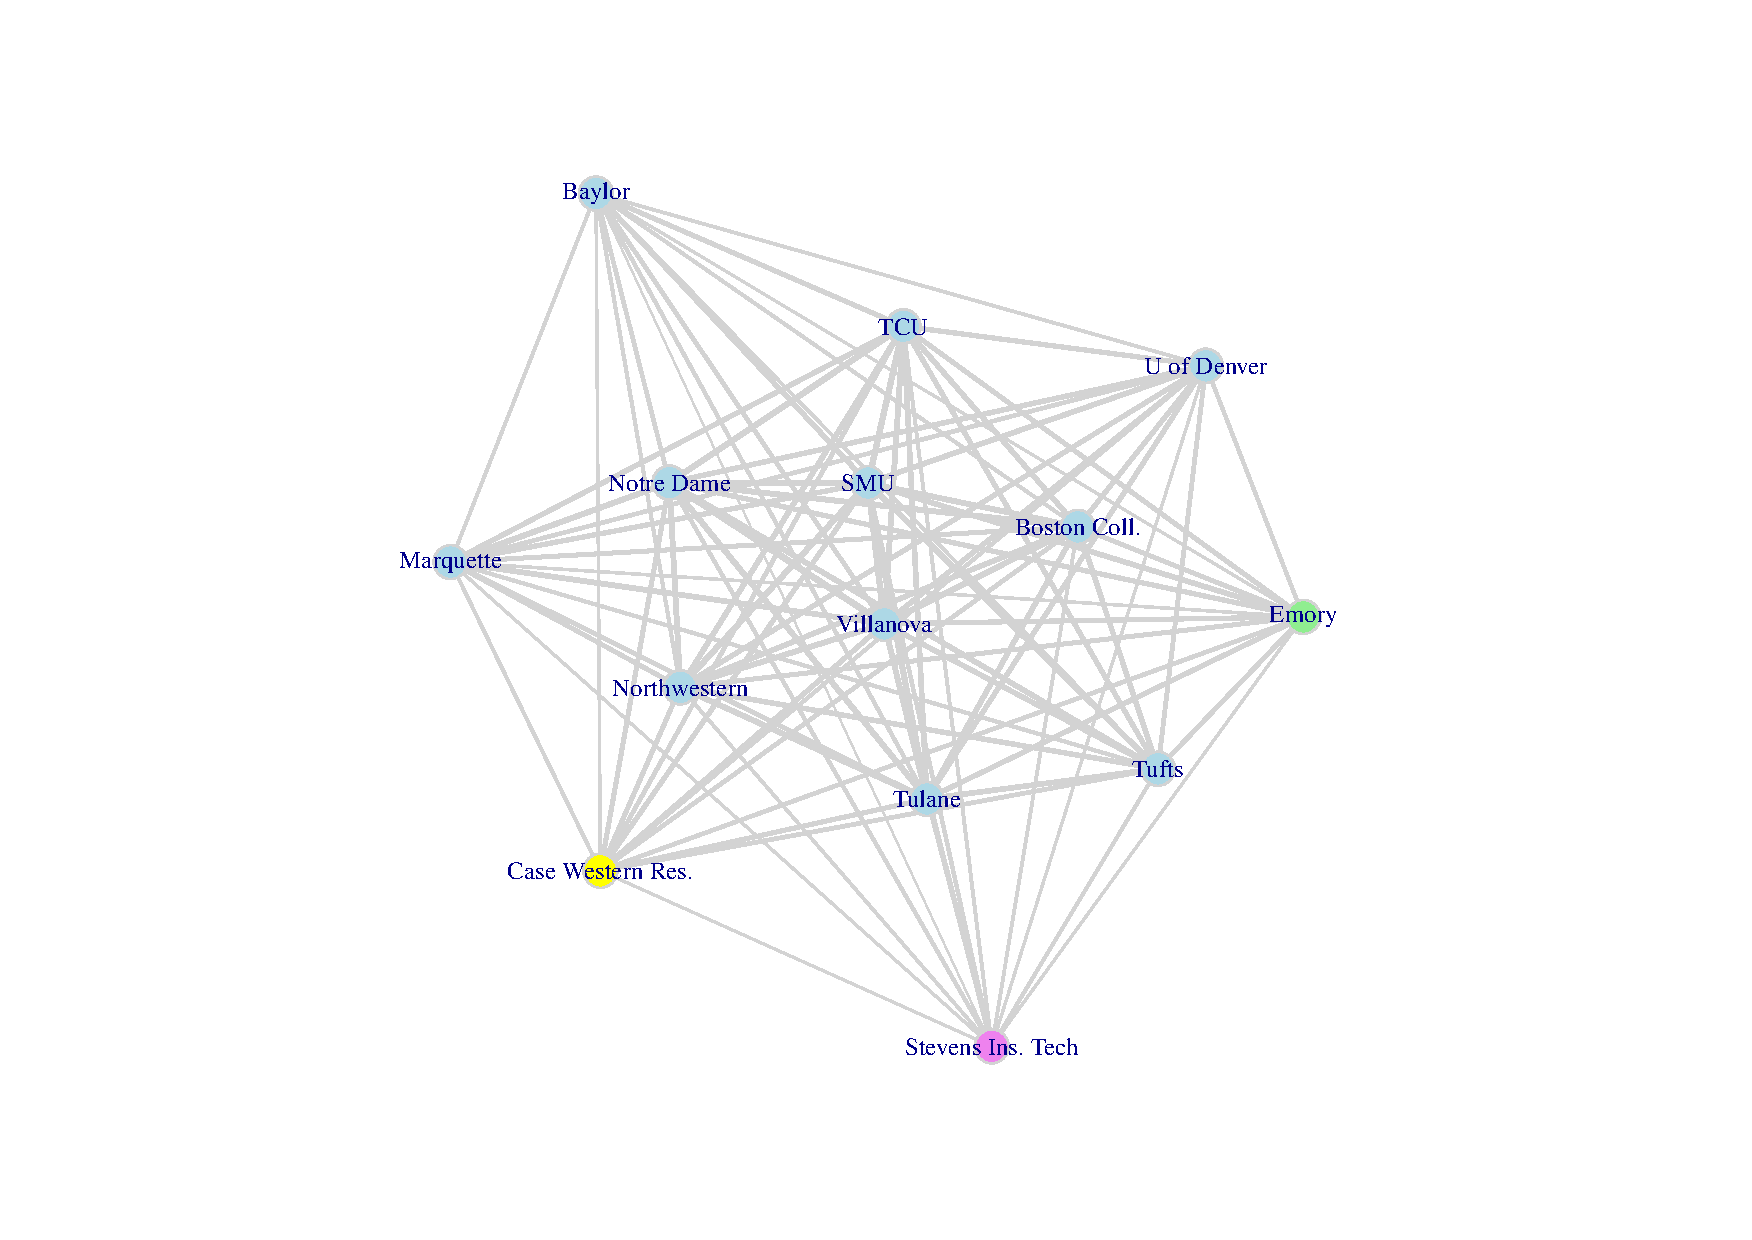
\includegraphics[width=2\linewidth]{../assets/figures/plot_1mode_privu} 

}

\caption{One-mode network for private universities, colored by cluster}\label{fig:plot-1mode-privu}
\end{figure}

\newpage


\begin{figure}

{\centering 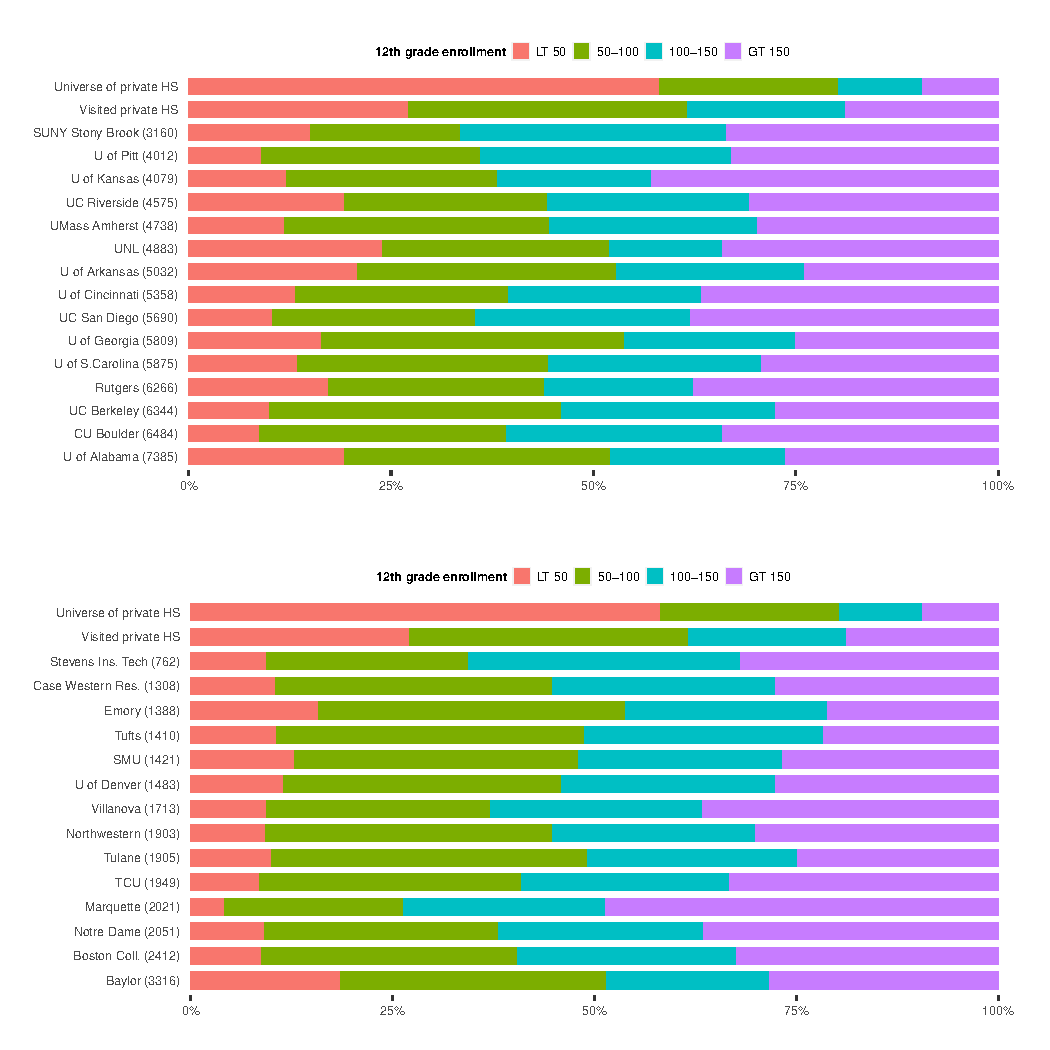
\includegraphics[width=2\linewidth]{../assets/figures/ego_network_enroll_pubu_privu} 

}

\caption{12th grade enrollment of visited private high schools}\label{fig:enroll-pubu-privu}
\end{figure}

\newpage

\begin{figure}

{\centering 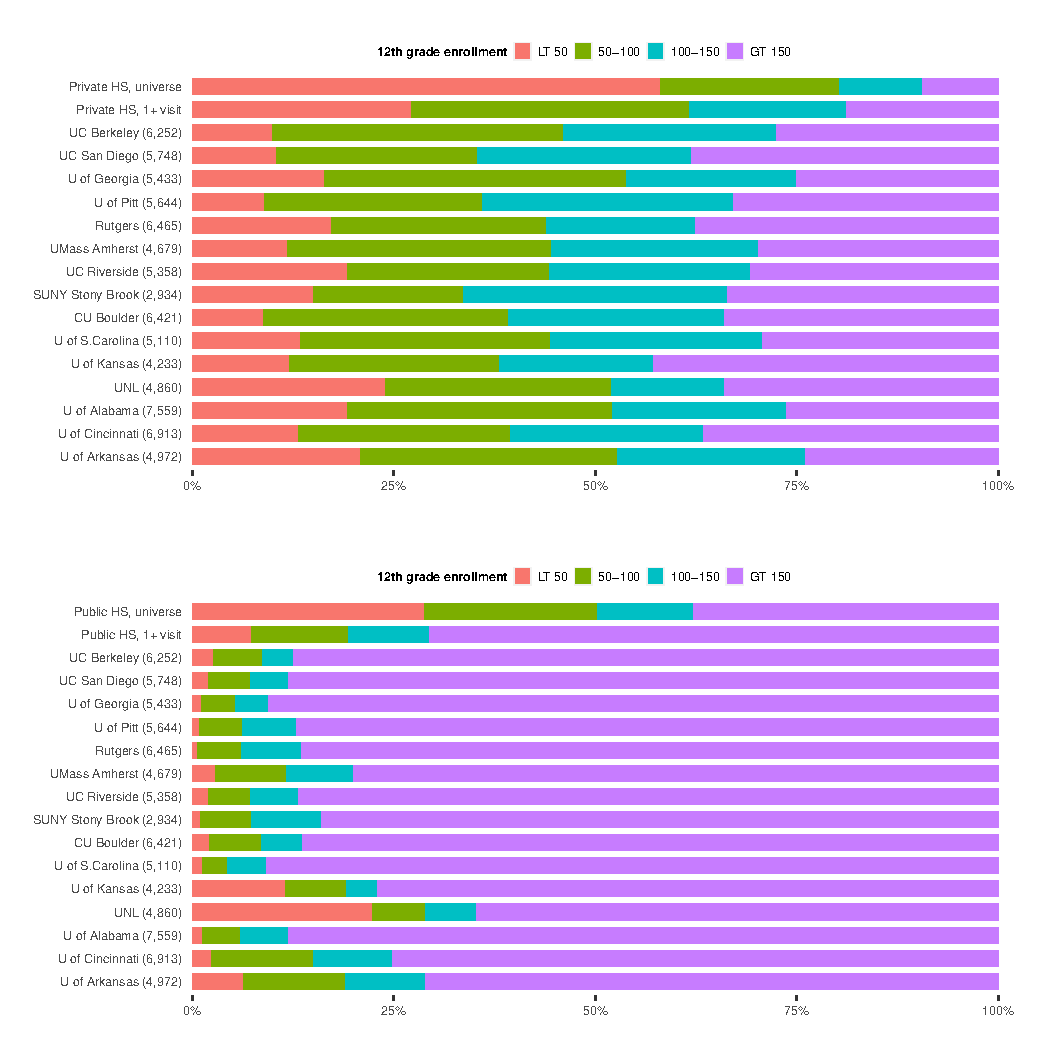
\includegraphics[width=2\linewidth]{../assets/figures/ego_network_enroll_pubu_privhs_pubhs} 

}

\caption{12th grade enrollment of visited private high schools vs. public high schools, public research universities}\label{fig:enroll-pubu-privhs-pubhs}
\end{figure}

\end{landscape}

\restoregeometry

\end{document}
